\documentclass[a4paper]{article}

%Packages
\usepackage{lmodern}
\usepackage{amsmath}	% advanced math symbols pkg
\usepackage{amsthm, amsthm}
\usepackage[utf8]{inputenc}	% utf8 encoding
\usepackage{graphicx} % pictures support
\usepackage{longtable} % table on multiple pages support
\usepackage[italian]{babel} % language support
\usepackage{enumitem} % custom enumeration support
\usepackage{rotating} % Rotating pictures support
\usepackage{float} % Support for floated images
\usepackage{hyperref} % Support for href in toc
\usepackage{marvosym} % Currency symbols
\usepackage{fancyhdr} % Fancy headers
\usepackage[a4paper]{geometry} % Geometry Page
\usepackage{array}
\usepackage{footnote}
\usepackage{setspace}
\usepackage{listings} % Code listings support
\usepackage[scaled]{beramono} % Monospace font

% Listings setup
\lstset{literate=%
{à}{{\`{a}}}1
{è}{{\`{e}}}1
{é}{{\'{e}}}1
{ì}{{\`{i}}}1
{ò}{{\`{o}}}1
{ù}{{\`{u}}}1
}
\lstset{extendedchars=\true}
\lstset{inputencoding=ansinew}
\lstset{language=SQL}
\lstset{basicstyle=\sffamily}

% Setup Hyperef
\hypersetup{
	colorlinks, 
	citecolor=black,
	filecolor=black,
	linkcolor=black,
	urlcolor=black
}

% Example tag definitions
\theoremstyle{definition}
\newtheorem{example}{Esempio}[section]

% layout setup
\headsep=50pt
\pagestyle{fancy}

% Defining frontespice
\newlength{\drop}% for my convenience
\setlength{\drop}{1em}
\newcommand*{\titleUnivpm}
{
	\begingroup
		\begin{center}
			{\Huge\bfseries\rmfamily Università Politecnica delle Marche}\\
			[\baselineskip]
		    \rule{\textwidth}{2pt}\par
		    \vspace*{\drop}
		    {\large\bfseries\rmfamily PROGETTAZIONE DI UNA BASE DI DATI}\\
		    {\large\bfseries\rmfamily PER}\\
		    {\Large\bfseries\rmfamily UN'OFFICINA MECCANICA}\\
		    \vspace*{2cm}
		    {\large\itshape\bfseries\rmfamily Relazione del Progetto per l'Esame di}\\
		    {\large\itshape\bfseries\rmfamily Sistemi Informativi e Basi di Dati}\\
	    \end{center}
	    \vspace*{2cm}   
	    \begin{minipage}{0.4\textwidth}
		    \begin{flushleft}
		    {\small\bfseries Docente di Riferimento:}\\
		    {\bfseries Professoressa}\\
		    {\bfseries\itshape Claudia DIAMANTINI }
		    \end{flushleft}
	    \end{minipage}
	    \begin{minipage}{0.4\textwidth}
		    \begin{flushright} 
		    {\bfseries\small Gruppo 809:}\\
		    {\bfseries\itshape Ilario Pierbattista}\\
		   	{\bfseries\itshape Alessandro Staffolani}\\
			{\bfseries\itshape Luka Petrovic}\\
		    \end{flushright}
	    \end{minipage}  
	    \vfill
	    \begin{center}
		    {\large\bfseries\rmfamily ANNO ACCADEMICO 2014-2015}
		\end{center}
    \endgroup
}

% Redefining arraystretch
\renewcommand{\arraystretch}{1.5}

\makeindex

%Document begin
\begin{document}

\titleUnivpm
\newpage

\tableofcontents
\newpage

% Introduzione
% \section{Introduzione}

	Consci dell'attuale situazione economica del nostro Paese e dell'importanza del ruolo che le piccole e medie imprese rivestono nell'economia locale\footnote{Province di Fermo, Macerata ed Ascoli Piceno}, siamo oltremodo convinti che, per combattere questo periodo di profonda crisi, l'innovazione tecnologica dei processi produttivi e dei sistemi informativi delle aziende sia un ingrediente fondamentale. Troppo spesso, nelle piccole realtà imprenditoriali, questo aspetto viene ignorato, comportando in molti casi enormi sprechi in termini di risorse temporali che potrebbero essere evitati.
	
	Abbiamo scelto di svillupare una base di dati per un'officina meccanica. È solamente una delle tante realtà imprenditoriali che il nostro territorio ospita, l'abbiamo scelta per la disponibità di contatti diretti con un professionista del settore.
	
	Lo scopo di questo elaborato è quello di tenere traccia delle fasi di sviluppo di questo progetto e quello di fornire una documentazione adeguata sulla base di dati.
% \newpage

% Sezione sull'analisi dei requisiti
\section{Analisi dei Requisiti}
\label{sec:req_analysis}

	Nessun elemento del team conosceva direttamente la realtà imprenditoriale di un'officina meccanica, ma abbiamo dei contatti con un professionista al quale abbiamo chiesto informazioni. 
	
	Per capire quali sono i requisiti della base di dati, abbiamo raccolto informazioni attraverso il nostro contatto, quindi abbiamo proceduto a raffinare tali informazioni strutturandole in modo che risultino adeguate a procedere all'effettiva progettazione.
	
	\subsection{Raccolta delle Informazioni}
		
		La raccolta delle informazioni è stata effettuata attraverso un'intervista al nostro contatto e grazie ad alcuni documenti che egli stesso ci ha messo a disposizione. 
	
		\subsubsection{Intervista}
		Abbiamo intervistato il \emph{Sig. Adriano Staffonali}, titolare di un'officina meccanica nel comune di Treia (MC). L'intervista risale al 26 Ottobre 2014. Riportiamo, qui di seguito, i passaggi fondamentali.

		% Intervista		
		\begin{description}
			\item[A] 
				Di cosa si occupa la sua attività?
			\item[AS] 
				\emph{La mia attività è un'officina meccanica. Mi occupo di effettuare piccole e medie riparazioni di tipo meccanico ad autovetture e sono specializzato nella sostituzione, riparazione e manutenzione dei componenti elettronici. Inoltre la mia officina è autorizzata all'installazione di impianti a metano e GPL "}Landi Renzo\emph{", azienda leader nel settore al livello nazionale.}
			\item[A]
				Quante persone vi lavorano?
			\item[AS]
				\emph{Attualmente solo io, ma in passato ho avuto un paio di dipendenti.}
			\item[A]
				Come si articola una tipica giornata di lavoro?
			\item[AS]
				\emph{Solitamente ho sempre degli impianti da installare, che occupano la maggior parte della giornata. Ho un calendario dove segno tutte le scadenze a cui devo tener fede. Quando arriva un cliente, che abbia bisogno di una riparazione all'auto o dell'installazione di un impianto, devo fornirgli un preventivo. Se accetta, controllo quali pezzi devo acquistare, rintraccio i fornitori e li ordino.}
			\item[A]
				Che tipo di clienti sono i suoi? Privati? Aziende? Come tiene traccia dei loro dati?
			\item[AS]
				\emph{Per lo più i miei clienti sono privati, ma mi capita di lavorare con aziende e - occasionalmente - anche con enti pubblici. Tengo traccia solamente dei clienti quando effettuano nuovi impianti, in quanto la} Landi Renzo \emph{richiede per ogni nuovo cliente una scheda d'installazione da compilare on-line contenente dati anagrafici, recapiti e dati  dell'autovettura.}
			\item[A]
				Ammesso di avere individuato il guasto e di aver ben presente quali sono i pezzi da sostituire, solitamente, quanto sono precisi i preventivi per una riparazione? E quelli per l'installazione di un impianto?
 			\item[AS]
 				\emph{Per quanto riguarda le riparazioni, non si può dare sempre un preventivo preciso. Bisogna tener conto di alcuni aspetti: l'uso di pezzi di ricambio originali o meno e le ore di lavoro necessarie per effettuare la riparazione (di cui è sempre difficile effettuare previsioni precise). Per quanto riguarda l'installazione di impianti, invece, l'azienda che li produce e me li fornisce, predispone un listino prezzi completo che mi permette di effettuare preventivi in modo veloce e accurato.}
 			\item[A]
 				Non tiene uno storico delle riparazioni effettuate al fine di riutilizzare i dati per trovare soluzioni più velocemente in futuro?
 			\item[AS]
 				\emph{Uno storico no. Ho alcuni schemi tecnici che mi aiutano a risolvere il problema più velocemente. Però uno storico sarebbe utile.}
 			\item[A]
	 			Cosa appunta in questi schemi?
	 		\item[AS]
		 		\emph{Una breve descrizione del malfunzionamento riscontrato, la causa principale del malfunzionamento, una lista con i pezzi che comunemente bisogna sostituire per eliminare il malfunzionamento e qualche appunto sul procedimento da seguire.}
		 	\item[A]
			 	Come identifica i componenti di ricambio necessari?
			\item[AS]
				\emph{Dipende dal componente. Alcuni, come le bombole per il metano, non vengono scelti in base al modello dell'auto, ma in base alle dimensioni e alla loro capacità. Altri invece dipendono dal modello dell'automobile, che siano originali o compatibili. Altre volte ancora il modello dell'automobile non è sufficiente, visto tra esemplari dello stesso modello alcuni pezzi possono cambiare. In quel caso faccio riferimento al sito del produttore dell'auto, facendo una ricerca in base al numero del telaio.}
 			\item[A]
 				Per quanto riguarda i pagamenti da parte dei clienti, come si è organizzato? Inoltre, permette pagamenti dilazionati o rateizzati da parte dei clienti, che essi siano privati od aziende?
 			\item[AS]
 				\emph{Al momento utilizzo un archivio cartaceo per quanto riguarda fatture e ricevute. Pagamenti dilazionati? Raramente. Solitamente i miei clienti mi lasciano un acconto iniziale, quando la cifra del preventivo è considerevole, alla fine del lavoro pagano il resto. Ad alcune aziende, con le quali intrattengo rapporti frequentemente, permetto di effettuare pagamenti dilazionati. Quando si tratta invece di enti pubblici (ho avuto in passato rapporti commerciali con il comune di Treia) il pagamento dilazionato è l'unica soluzione.}
 			\item[A]
 				E per quanto riguarda i suoi fornitori? Le permettono pagamenti dilazionati?
 			\item[AS]
 				\emph{A dire il vero, raramente. Essendo la mia una piccola azienda, solo alcuni fornitori con cui ho instaurato un rapporto di fiducia nel tempo, mi permettono pagamenti dilazionati.}
 			\item[A]
 				Quindi lei si occupa da solo anche di tutta la contabilità, giusto?
 			\item[AS]
 				\emph{Non del tutto. Ho un commercialista. Lui si occupa di stilare il Bilancio e lo Stato Patrimoniale.}
 			\item[A]
 				Lei è solito tenere in magazzino pezzi per alcune riparazioni frequenti?
 			\item[AS]
 				\emph{Sì, cerco di avere sempre disponibili i pezzi fondamentali.}
 			\item[A]
 				Riesce a gestire adeguatamente il magazzino? Le è mai capitato di avere avuto dei prodotti che, soggetti magari all'usura del tempo, si siano rovinati?
 			\item[AS]
 				\emph{Ci sono alcuni prodotti che sono più soggetti di altri all'usura del tempo, altri invece che diventano obsoleti. Faccio un inventario completo delle rimanenze in magazzino una volta all'anno ed è un'attività che porta via molto tempo. Inoltre, quando utilizzo un pezzo per una riparazione, non vado ad aggiornare l'inventario, quindi non riesco a sapere ogni volta con precisione lo stato del magazzino.}
 			\item[A]
 				Per quanto riguarda i dati dei fornitori come ne tiene traccia? È sempre in grado di ritrovarli facilmente e immediatamente?
 			\item[AS]
 				\emph{Sinceramente no, non di tutti i dati. Se ne occupa il mio commercialista. Io ho solamente una rubrica cartacea con i numeri di telefono. Infatti, quando ho bisogno di dati che non siano i semplici numeri telefonici, devo contattare lui. Alcuni fornitori mi inviano le loro fatture via e-mail e queste contengono i dati dell'azienda di riferimento, ma anche in questo caso non è sempre agevole ritrovarli quando servono.}
 			\item[A]
 				Lei lavora da solo, ma ha detto di aver avuto un dipendente. Che tipo di contratto aveva? Si occupava personalmente delle buste paga?
 			\item[AS]
 				\emph{Giornalmente segnavo le sue ore di lavoro, quindi gli versavo l'importo a fine mese. Riuscivo ad occuparmene tranquillamente, era un solo dipendente d'altronde, ma se in futuro avessi bisogno di assumere più di una persona, dovrei adottare un altro metodo.}
		\end{description}
				
		\subsubsection{Documenti raccolti}
			Aggiungere le immagini dei documenti raccolti
			
		\subsubsection{Analisi dei processi interni}
			
			Abbiamo realizzato uno schema informale (figura \ref{fig:internal_processes}) che descrive il flusso dei dati all'effettuarsi delle procedure tipiche dell'attività.
			
			
			\begin{sidewaysfigure}
				\centering
				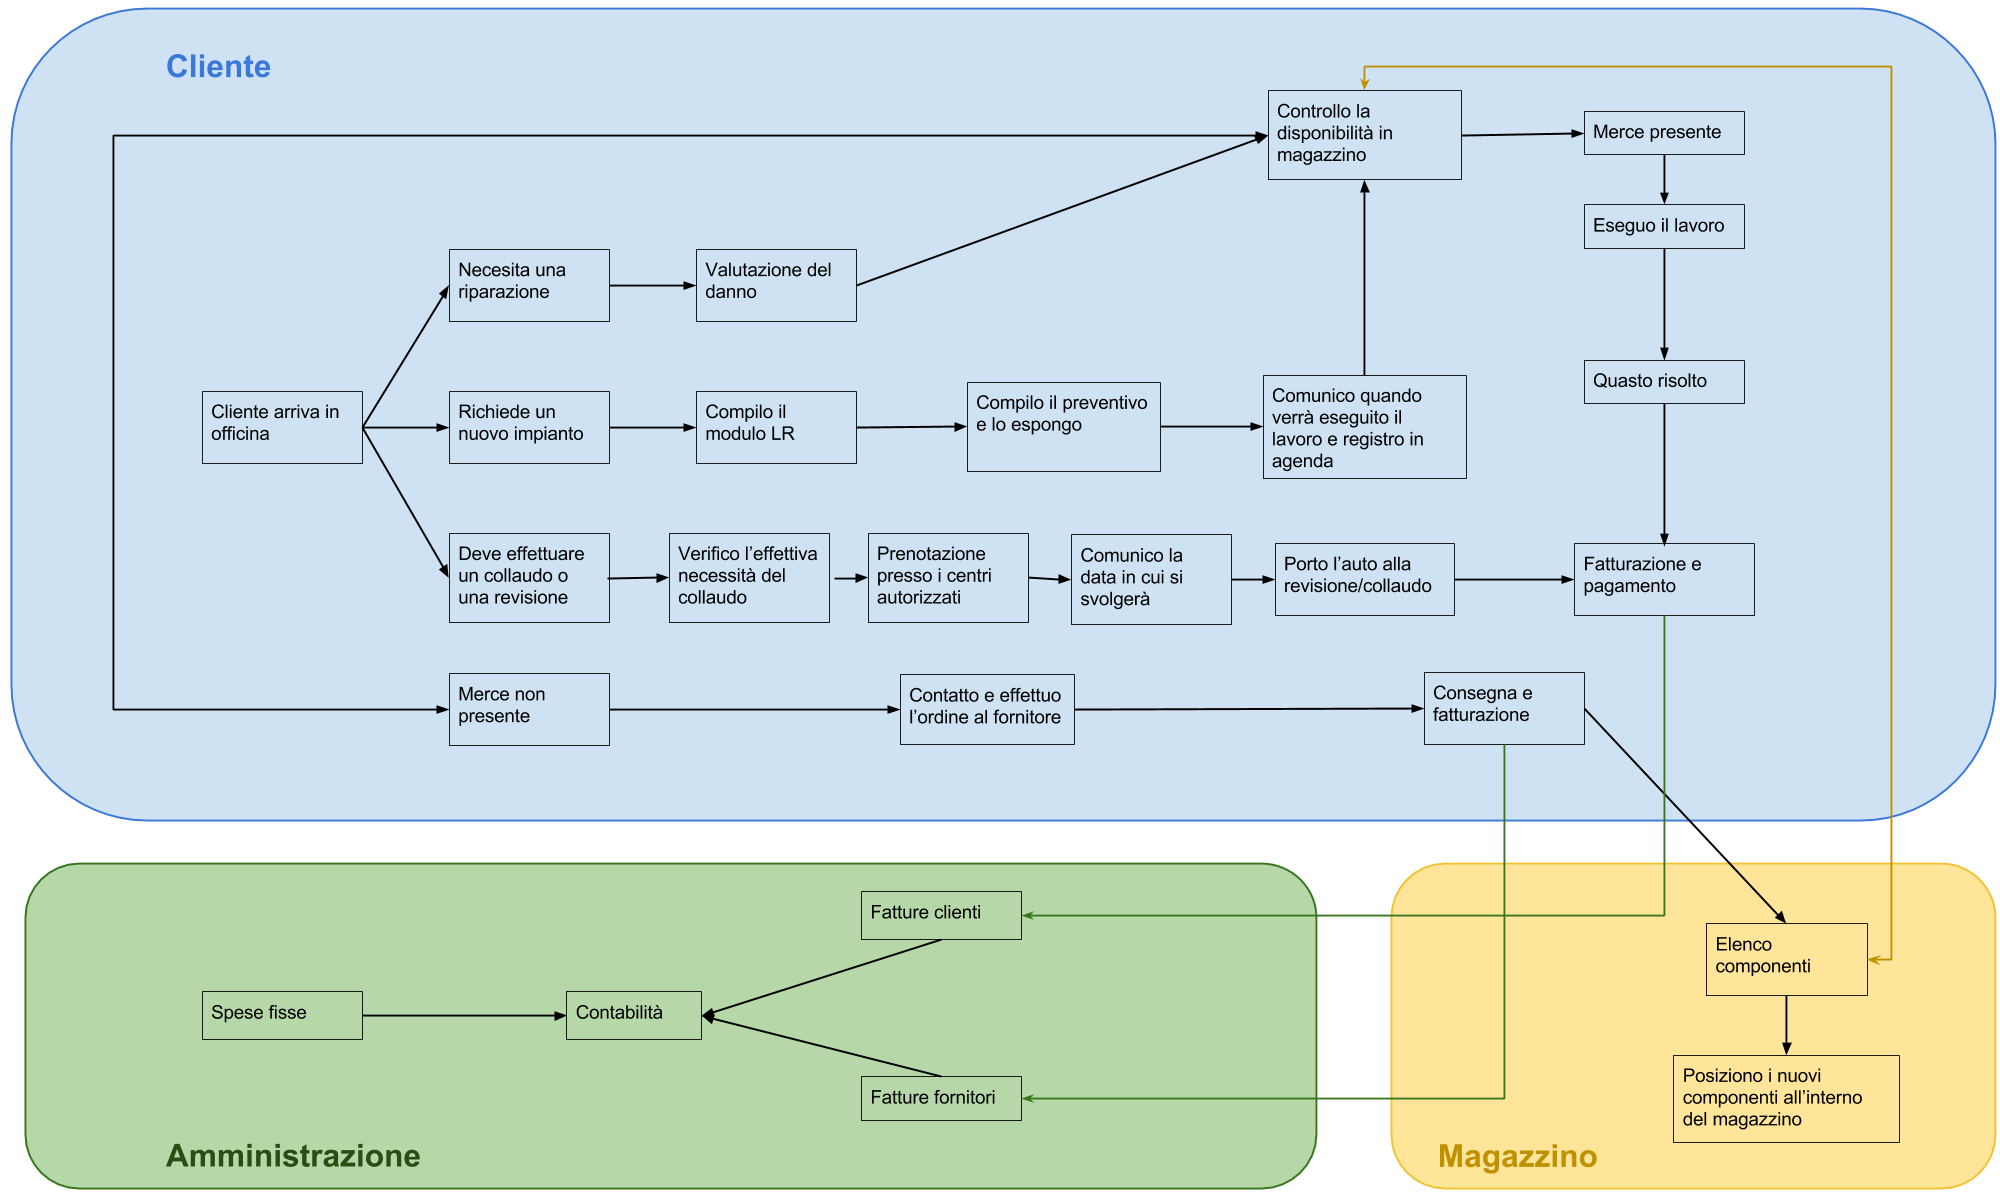
\includegraphics[width=22cm]{images/internal_processes.png}
				\caption{Analisi dei Processi Interni}
				\label{fig:internal_processes}
			\end{sidewaysfigure}
		
	\subsection{Requisiti Espressi nel Linguaggio Naturale}
	
		A partire dall’analisi dell’intervista e dall’analisi dei documenti in nostro possesso, abbiamo elaborato quelli che sono, a nostro avviso, i requisiti della base di dati che andremo a sviluppare.
		
		Il nostro obbiettivo è quello di sviluppare una base di dati per la gestione di un’officina meccanica di piccole medie dimensioni specializzata nell’installazione di impianti a metano e a GPL, ma che effettua anche riparazioni di natura meccanica ed elettronica alle autovetture.
		
		Bisognerà gestire i dati riguardanti i clienti e le loro autovetture, quelli riguardanti i fornitori e dei dipendenti. Bisognerà tenere traccia dei componenti presenti in magazzino, degli ordini effettuati e delle forniture ricevute.
		Si vuole tenere traccia dei dati riguardanti i preventivi emessi dall'attività e affiancandoli ai dati riguardanti le prestazioni effettuate a capo di tali preventivi, fornendo così uno storico consultabile delle attività effettuate nel tempo dall'azienda. Con il passare del tempo, tale storico diventerà una valida risorsa da cui attingere per agevolare il processo di formulazione dei preventivi, nonchè per rendere questi ultimi più precisi.
		Si vogliono conoscere i componenti più utilizzati nelle riparazioni e nelle installazioni, al fine di stabilire dei quantitativi minimi per ciascuno di essi da avere sempre a disposizione nel magazzino. Inoltre, si vuole fare in modo di evitare gli sprechi dovuti a componenti che diventano obsoleti o che si rovinano a causa dell'usura.
		Si vuole anche tenere traccia delle transazioni monetarie entranti (pagamenti dei clienti per le prestazioni ricevute) ed uscenti (versamenti ai fornitori ed ai dipendenti).
		
		Per quanto riguarda i clienti non dotati di partita iva, si vogliono conoscere il codice fiscale, il nome, il cognome, l’indirizzo di residenza, i vari recapiti. Per i clienti forniti di partita iva, si vuole tener traccia, appunto, della partita iva, della ragione sociale e dell’indirizzo della sede legale. 
		Nel caso in cui un cliente non dotato di partita iva richieda l’installazione di un nuovo impianto, sarà necessario conoscere anche il codice identificativo del documento di identità per le comunicazioni con la Motorizzazione Civile.
		
		Per quanto riguarda le autovetture sarà necessario conoscere la targa, la marca, il nome del modello, il numero del telaio. Se per un’autovettura viene richiesta l’installazione di un impianto, sarà necessario conoscere anche la cilindrata, l’anno di immatricolazione e la data dell’ultima revisione. Ad installazione eseguita sarà necessario aggiungere anche la data in cui l'impianto viene collaudato.
		
		A proposito dei fornitori, sarà necessario conoscerne la partita via, la ragione sociale, i vari recapiti, i tempi medi di consegna, la modalità di pagamento preferita (bonifico bancario o assegno) ed - eventualmente - il codice IBAN.
		
		Dei dipendenti si vuole tener traccia di codice fiscale, nome, cognome, luogo di nascita, data di nascita, indirizzo di residenza, retribuzione oraria (ove il dipendente venga pagato in base alle ore di lavoro effettuate), stipendio mensile (ove invece il dipendente abbia un contratto che prevede una retribuzione mensile costante), modalità di riscossione ed - eventualmente - il codice IBAN. Si vogliono anche conoscere le presenze che i dipendenti effettuano, tenendo conto dell’ora di inizio del turno, l’ora di fine e la data di rifermento. 
		L'inserimento degli orari di inizio e di fine del turno può essere effettuata manualmente dal titolare alla fine della giornata oppure tramite l'installazione di un dispositivo di lettura di badge magnetici.
		
		Riguardo ai componenti si vogliono conoscere il nome, il tempo di validità dal momento dell'acquisto (dopo il quale il componente risulta rovinato dall'usura o diviene obsoleto), il prezzo di vendita e la quantità minima che deve essere sempre presente nel magazzino.
		
		L'acquisto dei componenti viene formalizzato attraverso un ordine. Un ordine sarà composto da una o più forniture, dalla partita iva del fornitore presso cui si fa l'ordine, dalla data in cui l'ordine viene effettuato e dalla data in cui è stata consegnata la merce.
		
		Per fornitura si intende un insieme omogeneo di componenti acquistati nello stesso ordine. Ognuna di esse sarà caratterizzata dal componente, dalla quantità acquistata e dal prezzo unitario di acquisto.
		
		Per quanto riguarda la gestione del magazzino, al fine di evitare che alcuni componenti diventino obsoleti o si rovinino con il tempo, bisogna fare in modo che vengano utilizzati prima quelli la cui \emph{data di scadenza} è più prossima di altri. Per fare ciò, conoscendo il periodo di validità del componente, sarà necessario avere anche la data d'acquisto.
		Possiamo considerare il magazzino come un elenco di \emph{forniture attive}, ovvero una fornitura i cui componenti non siano già stati tutti utilizzati. Affiancando alla fornitura di riferimento, la quantità rimanente dei componenti di quella fornitura, avremo tutti i dati necessari.
		
		Riguardo i preventivi sarà necessario conoscere innanzi tutto la categoria dell'intervento richiesto (riparazione, installazione di un impianto a metano, installazione di un impianto a gpl, collaudo, revisione). Serviranno inoltre la data di emissione del preventivo, la data in cui dovrebbe cominciare il lavoro, i componenti che si prevede saranno utilizzati per compiere il lavoro, la stima dei costi della manodopera, la stima dei costi di eventuali servizi aggiuntivi e l'ammontare di un eventuale acconto versato dal cliente.
		Nel caso in cui il cliente necessiti di una riparazione sarà utile aggiungere una brevissima descrizione dei sintomi.
		Se il cliente necessita dell’installazione di un nuovo impianto, sarà necessario tenere conto anche della tipologia del sistema di alimentazione (iniezione o aspirazione). Inoltre, per avere la completa compatibilità con il modello per i preventivi imposti dall'azienda \emph{Landi Renzo}, di ogni componente necessario per effettuare l'installazione di un impianto, sarà necessario conoscere la relativa ubicazione nell'autovettura, facendo distinzione tra i componenti necessari per il vano motore e quelli per il vano bagagliaio.
		
		Riguardo le prestazioni, eseguite a fronte di un preventivo, si vuole conoscere il preventivo di riferimento, i tempi effettivi di esecuzione, la data in cui è stato finito il lavoro, i componenti che sono stati effettivamente utilizzati, costo manodopera, il costo di eventuali servizi aggiuntivi, i lavoratori che hanno le hanno eseguite.
		Nel caso di riparazioni è utile aggiungere anche una brevissima descrizione del danno riscontrato ed una descrizione più approfondita sul procedimento utilizzato per effettuare la riparazione.
		
		Ad ogni prestazione fa capo una fattura. I dati delle fatture di cui è importante tener traccia sono il numero progressivo di fattura (da azzerare all'inizio di ogni anno), la data di emissione, l'ammontare dell'imponibile, l'ammontare delle imposte, ammontare di un eventuale sconto, ammontare di eventuali incentivi il sistema di pagamento (rimessa diretta o rimessa differita), il tipo di pagamento (assegno, bonifico o contanti), lo stato del pagamento. Nel caso di pagamenti con rimessa differita sarà necessario conoscere anche la data di scadenza.
		
		Si vogliono conoscere anche i dati relativi alle transazioni monetarie, entranti o uscenti che siano. Nel dettaglio, si vuole tener traccia della quota delle singole transazioni e della data di emissione.
		
	\subsection{Glossario dei Termini}
	
		Al fine di evitare la presenza di ambiguità, abbiamo stilato un glossario dei termini più importanti a cui faremo riferimento di qui in avanti.
						
		\begin{longtable}{| p{2.5cm} | p{4.5cm} | p{2cm} | p{2.5cm} |}
				
			\hline
			\textbf{Termine} & 
			\textbf{Descrizione} & 
			\textbf{Sinonimi} & 
			\textbf{Collegamenti} \\
			
			\endfirsthead
				
			\hline
			\textbf{Termine} & 
			\textbf{Descrizione} & 
			\textbf{Sinonimi} & 
			\textbf{Collegamenti} \\
			
			\endhead
			
			\hline
			Cliente & 
			Persona fisica o giuridica che abbia avuto rapporti con l'azienda.
			&&\\ \hline
			Autovettura &
			Automobile di un cliente che debba subire o abbia già subito un intervento da parte dei lavoratori dell’azienda. &
			Automobile, Veicolo &
			Cliente, Preventivo
			\\ \hline
			Preventivo &
			Stima dei costi, dei tempi e dei componenti necessari relativi all’esecuzione di un intervento su un’autovettura. & &
			Autovettura, Componente, Prestazione
			\\ \hline
			Preventivo di Riparazione &
			Preventivo relativo alla riparazione di un guasto di un’autovettura & &
			Preventivo 
			\\ \hline
			Preventivo d'Installazione & 
			Preventivo relativo all’installazione di un nuovo impianto in un’autovettura. & &
			Preventivo
			\\ \hline
			Componente &
			Qualsiasi oggetto fisico necessario alla corretta esecuzione di una riparazione o di una installazione di un impianto su di un’autovettura &
			Prodotto &
			Fornitore, Prestazione, Preventivo
			\\ \hline
			Fornitore & 
			Azienda che abbia fornito all’officina qualsiasi tipo di componente necessario. & &
			Componente, Fornitura
			\\ \hline
			Ordine &
			Insieme di componenti acquistati presso un fornitore. I componenti omogenei sono organizzati in forniture. &
			&
			Componente, Fornitura
			\\ \hline
			Fornitura & 
			Insieme omogeneo di componenti acquistati presso un fornitore nel medesimo ordine. &
			&
			Componente, Fornitore
			\\ \hline
			Magazzino &
			Insieme totale dei componenti depositati fisicamente in una apposita area nei locali utilizzati dall'attività in attesa di essere utilizzati. &
			Deposito &
			Componente, Fornitura Attiva
			\\ \hline
			Fornitura Attiva &
			Si fa riferimento a quelle forniture i cui componenti, totalmente o in parte, sono ancora presenti in magazzino in attesa di essere utilizzati. &
			&
			Componente, Fornitura, Magazzino
			\\ \hline
			Data di scadenza &
			Riferito ad un componente è la data, calcolata a partire da quella d'acquisto, oltre il quale il componente diventa inutilizzabile per obsolescenza o per usura. &
			&
			Componente
			\\ \hline
			Dipendente & 
			Persona fisica che abbia lavorato per l’officina &
			Lavoratore, Operatore &
			\\ \hline
			Transazione &
			Flusso di denaro uscente o entrante nella cassa dell’attività. &
			Flusso di Cassa &
			\\ \hline
			Prestazione &
			Attività eseguita dai lavoratori dell’officina su di un’autovettura. & &
			Preventivo
			\\ \hline
			Sintomo &
			Malfunzionamento direttamente verificabile di un autoveicolo, individuabile senza il bisogno di conoscerne le cause. &
			& \\ \hline
			Pagamento &
			Transazione di denaro entrante a seguito di una prestazione fornita ad un cliente. &&
			Prestazione, Transazione
			\\ \hline
			Versamento &
			Transazione di denaro uscente a seguito di una fornitura ricevuta o di uno stipendio versato ad un dipendente. & 
			Spesa & 
			Transazione, Fornitore, Dipendente 
			\\ \hline
			Collaudo &
			Attività relativa alla verifica specifica del corretto funzionamento del serbatoio installato con il nuovo impianto (che sia a metano o gpl). &&
			Autovettura
			\\ \hline
			Revisione & 
			Attività di verifica del corretto funzionamento dei tutte le parti dell’autovettura. &&
			Autovettura
			\\ \hline
			Retribuzione Oraria & 
			Ammontare della retribuzione di un dipendente per ogni ora di lavoro. && 
			Dipendente
			\\ \hline
			Modalità di Riscossione &
			Modalità, indicata dal dipendente, con cui quest’ultimo riceve lo stipendio. &&
			Dipendente 
			\\ \hline
			Impianto & 
			Infrastruttura di alimentazione di un’autovettura.
			&&\\ \hline
			Imponibile &
			Somma di denaro su cui vanno calcolate le imposte previste per legge. &&
			Pagamento 
			\\ \hline
			Rimessa diretta &
			Si intende il sistema di pagamento nel quale la prestazione viene pagata immediatamente dopo la consegna della fattura &
			& \\ \hline
			Rimessa differita &
			Si intende il sistema di pagamento nel quale la prestazione viene pagata dal cliente entro 30, 60 o 90 giorni dalla consegna della fattura. &
			& \\ \hline
			Tipo di pagamento &
			Modalità di trasferimento di denaro. &
			& \\ \hline
				
		\end{longtable}
		
	\subsection{Eliminazione delle Ambiguità Presenti}
		
		Potrebbe risultare ambiguo l'utilizzo che viene fatto del termine \emph{componente}. Ci si riferisce, con componente, ad un oggetto fisico necessario all'esecuzione di una prestazione, ma viene usato anche per identificare la classe stessa dell'oggetto, piuttosto che l'oggetto singolo.
		
		Si propone la seguente precisazione:
		\begin{description}
			\item[Componente]
				Classe di oggetti reali necessari ad effettuare una prestazione.
			\item[Articolo]
				Oggetto fisico necessario ad effettuare una prestazione.
		\end{description}
		
		\begin{example}
			Nel magazzino ci sono 10 bombole da 50 litri. Si dirà che nel magazzino sono presenti 10 articoli del componente "bombola da 50 litri".
		\end{example}
		
		Apporteremo, ove necessario, le correzioni nella sezione successiva.
		
	\subsection{Strutturazione dei Requisiti}
	
		\subsubsection{Frasi di Carattere Generale}
					
			Bisognerà gestire i dati riguardanti i clienti e le loro autovetture, quelli riguardanti i fornitori e dei dipendenti. Bisognerà tenere traccia dei componenti presenti in magazzino, degli ordini effettuati e delle forniture ricevute.
			Si vuole tenere traccia dei dati riguardanti i preventivi emessi dall'attività e affiancandoli ai dati riguardanti le prestazioni effettuate a capo di tali preventivi, fornendo così uno storico consultabile delle attività effettuate nel tempo dall'azienda. Con il passare del tempo, tale storico diventerà una valida risorsa da cui attingere per agevolare il processo di formulazione dei preventivi, nonchè per rendere questi ultimi più precisi.
			Si vogliono conoscere i componenti più utilizzati nelle riparazioni e nelle installazioni, al fine di stabilire dei quantitativi minimi per ciascuno di essi da avere sempre a disposizione nel magazzino. Inoltre, si vuole fare in modo di evitare gli sprechi dovuti a componenti che diventano obsoleti o che si rovinano a causa dell'usura.
			Si vuole anche tenere traccia delle transazioni monetarie entranti (pagamenti dei clienti per le prestazioni ricevute) ed uscenti (versamenti ai fornitori ed ai dipendenti).
			
			L'acquisto dei componenti viene formalizzato attraverso un ordine.
			
		\subsubsection{Frasi relative ai Clienti}
		
			Per quanto riguarda i clienti non dotati di partita iva, si vogliono conoscere il codice fiscale, il nome, il cognome, l’indirizzo di residenza, i vari recapiti. Per i clienti forniti di partita iva, si vuole tener traccia, appunto, della partita iva, della ragione sociale e dell’indirizzo della sede legale. 
			Nel caso in cui un cliente non dotato di partita iva richieda l’installazione di un nuovo impianto, sarà necessario conoscere anche il codice identificativo del documento di identità per le comunicazioni con la Motorizzazione Civile.
		
		\subsubsection{Frasi relative alle Autovetture}
			
			Per quanto riguarda le autovetture sarà necessario conoscere la targa, la marca, il nome del modello, il numero del telaio. Se per un’autovettura viene richiesta l’installazione di un impianto, sarà necessario conoscere anche la cilindrata, l’anno di immatricolazione e la data dell’ultima revisione. Ad installazione eseguita sarà necessario aggiungere anche la data in cui l'impianto viene collaudato.
		
		\subsubsection{Frasi relative ai Fornitori}
			
			A proposito dei fornitori, sarà necessario conoscerne la partita via, la ragione sociale, i vari recapiti, i tempi medi di consegna, la modalità di pagamento preferita (bonifico bancario o assegno) ed - eventualmente - il codice IBAN.
		
		\subsubsection{Frasi relative ai Dipendenti} 
			
			Dei dipendenti si vuole tener traccia di codice fiscale, nome, cognome, luogo di nascita, data di nascita, indirizzo di residenza, retribuzione oraria (ove il dipendente venga pagato in base alle ore di lavoro effettuate), stipendio mensile (ove invece il dipendente abbia un contratto che prevede una retribuzione mensile costante), modalità di riscossione ed - eventualmente - il codice IBAN. Si vogliono anche conoscere le presenze che i dipendenti effettuano, tenendo conto dell’ora di inizio del turno, l’ora di fine e la data di rifermento. 
			L'inserimento degli orari di inizio e di fine del turno può essere effettuata manualmente dal titolare alla fine della giornata oppure tramite l'installazione di un dispositivo di lettura di badge magnetici.
			
		\subsubsection{Frasi relative ai Componenti}
			
			Riguardo ai componenti si vogliono conoscere il nome, il tempo di validità dal momento dell'acquisto (dopo il quale il componente risulta rovinato dall'usura o diviene obsoleto), il prezzo di vendita e la quantità minima che deve essere sempre presente nel magazzino.
			
		\subsubsection{Frasi relative agli Ordini}
		
			L'acquisto dei componenti viene formalizzato attraverso un ordine. Un ordine sarà composto da una o più forniture, dalla partita iva del fornitore presso cui si fa l'ordine, dalla data in cui l'ordine viene effettuato e dalla data in cui è stata consegnata la merce.
		
		\subsubsection{Frasi relative alle Forniture}
		
			Per fornitura si intende un insieme di articoli dello stesso componente acquistati nello stesso ordine. Ognuna di esse sarà caratterizzata dal componente, dalla quantità acquistata e dal prezzo unitario di acquisto.
			
		\subsubsection{Frasi relative al Magazzino}
			
			Per quanto riguarda la gestione del magazzino, al fine di evitare che alcuni articoli diventino obsoleti o si rovinino con il tempo, bisogna fare in modo che vengano utilizzati prima quelli la cui \emph{data di scadenza} è più prossima di altri. Per fare ciò, conoscendo il periodo di validità del componente, sarà necessario avere anche la data d'acquisto dell'articolo.
			Possiamo considerare il magazzino come un elenco di \emph{forniture attive}, ovvero una fornitura i cui articoli non siano già stati tutti utilizzati. Affiancando alla fornitura di riferimento, la quantità rimanente degli articoli di quella fornitura, avremo tutti i dati necessari.
			
		\subsubsection{Frasi relative ai Preventivi}
		\label{sec:frasi_preventivi}
			
			Riguardo i preventivi sarà necessario conoscere innanzi tutto la categoria dell'intervento richiesto (riparazione, installazione di un impianto a metano, installazione di un impianto a gpl, collaudo, revisione). Serviranno inoltre la data di emissione del preventivo, la data in cui dovrebbe cominciare il lavoro, i componenti che si prevede saranno utilizzati per compiere il lavoro, la stima dei costi della manodopera, la stima dei costi di eventuali servizi aggiuntivi e l'ammontare di un eventuale acconto versato dal cliente.
			Nel caso in cui il cliente necessiti di una riparazione sarà utile aggiungere una brevissima descrizione dei sintomi.
			Se il cliente necessita dell’installazione di un nuovo impianto, sarà necessario tenere conto anche della tipologia del sistema di alimentazione (iniezione o aspirazione). Inoltre, per avere la completa compatibilità con il modello per i preventivi imposti dall'azienda \emph{Landi Renzo}, di ogni componente necessario per effettuare l'installazione di un impianto, sarà necessario conoscere la relativa ubicazione nell'autovettura, facendo distinzione tra i componenti necessari per il vano motore e quelli per il vano bagagliaio.
			
		\subsubsection{Frasi relative alle Prestazioni}
		
			Riguardo le prestazioni, eseguite a fronte di un preventivo, si vuole conoscere il preventivo di riferimento, i tempi effettivi di esecuzione, la data in cui è stato finito il lavoro, i componenti che sono stati effettivamente utilizzati, costo manodopera, il costo di eventuali servizi aggiuntivi, i lavoratori che hanno le hanno eseguite.
			Nel caso di riparazioni è utile aggiungere anche una brevissima descrizione del danno riscontrato ed una descrizione più approfondita sul procedimento utilizzato per effettuare la riparazione.
			
		\subsubsection{Frasi relative alle Fatture}
		
			Ad ogni prestazione fa capo una fattura. I dati delle fatture di cui è importante tener traccia sono il numero progressivo di fattura (da azzerare all'inizio di ogni anno), la data di emissione, l'ammontare dell'imponibile, l'ammontare delle imposte, ammontare di un eventuale sconto, ammontare di eventuali incentivi il sistema di pagamento (rimessa diretta o rimessa differita), il tipo di pagamento (assegno, bonifico o contanti), lo stato del pagamento. Nel caso di pagamenti con rimessa differita sarà necessario conoscere anche la data di scadenza.
		
		\subsubsection{Frasi relative alle Transazioni}
		
			Si vogliono conoscere anche i dati relativi alle transazioni monetarie, entranti o uscenti che siano. Nel dettaglio, si vuole tener traccia della quota delle singole transazioni e della data di emissione.
			
	\subsection{Specifica delle Operazioni}
		
		Abbiamo individuato le operazioni che, con lo sviluppo di tale base di dati, si intendono svolgere sulla stessa. Abbiamo aggiunto ad ogni operazione una stima della frequenza con la quale l'operazione stessa viene effettuata.
		
		Non sono presenti operazioni di cancellazione. Quest'ultime infatti sono previste solo nel caso in cui vengano commessi degli errori in fase di inserimento.
	
		\setenumerate[1]{label=OP\arabic*:}
		\begin{enumerate}
			
			% Inserimenti
			\item Inserimento di un nuovo cliente (3 volte a settimana)
			\item Inserimento di una nuova autovettura (3 volte a settimana)
			\item Inserimento di un nuovo fornitore (4 volte all’anno)
			\item Inserimento di un nuovo componente (2 volte al mese)
			\item Inserimento di un nuovo ordine (2 volta a settimana)
			\item Inserimento di una nuova fornitura (10 volte a settimana)
			\item Inserimento di un nuovo preventivo (10 volte a settimana)
			%\item Inserimento di un nuovo preventivo per l’installazione di un impianto (3 volte a settimana)
			%\item Inserimento di un nuovo preventivo per una riparazione (7 volte a settimana)
			\item Inserimento di una nuova prestazione (10 volte a settimana)
			\item Inserimento di una nuova fattura (10 volte a settimana)
			\item Inserimento di un nuovo dipendente (1 volta all’anno)
			\item Inserimento di un nuovo recapito (1 volta per ogni nuovo cliente e per ogni dipendente, in media 2 volte per ogni nuovo fornitore)
			\item Inserimento di una nuova presenza (1 volta al giorno per ogni dipendente)
			\item Inserimento di una nuova transazione (1 volta ogni 2 preventivi, 1 volta al mese per ogni dipendente, 1 volta per ogni fornitura, 1 volta per ogni prestazione)
			
			% Assegnazioni
			\item Assegnazione di un componente ad un preventivo (6 volte per ogni preventivo)
			\item Assegnazione di un componente ad una prestazione (6 volte per ogni prestazione)
			
			% Aggiornamento
			\item Modifica dei dati di un cliente (2 volte l’anno)
			\item Modifica dei dati di un fornitore (1 volta l’anno)
			\item Modifica dei dati di un dipendente (1 volta l’anno)
			\item Modifica del prezzo di vendita di un componente (1 volta al mese)
			
			% Consultazione
			\item Consultazione della data dell’ultimo collaudo per un’autovettura (1 volte a settimana)
			\item Consultazione della data dell’ultima revisione per un’autovettura (1 volte a settimana)
			\item Consultazione delle transazioni avvenute in un certo periodo (1 volta a settimana)
			\item Consultazione dello storico delle riparazioni (2 volte al giorno)
			\item Consultazione dello storico dei preventivi (2 volte al giorno)
			\item Consultazione della disponibilità di un componente (4 volte al giorno)
			\item Consultazione delle presenze di un dipendente in un arco temporale (1 volta al mese)
			\item Consultazione della lista dei componenti presenti (1 volta al mese)
			\item Consultazione della lista dei componenti più usati (2 volte al mese)
			\item Consultazione della lista dei componenti che si dovrebbero acquistare nuovamente (1 volta a settimana)
			\item Consultazione della lista dei recapiti per un cliente (1 volta al giorno)
			\item Consultazione della lista dei recapiti per un fornitore (1 volta a settimana)
			\item Consultazione della lista dei recapiti per un dipendente (1 volta a settimana)
			\item Consultazione della lista delle fatture che devono essere ancora pagate (1 volta al giorno)
			\item Consultazione della lista dei lavori da eseguire (2 volta al giorno)
			\item Consultazione dei dati per stilare una fattura o una ricevuta fiscale (10 volte a settimana)
			\item Calcolo dello stipendio per un dipendente (1 volta al mese)
			\item Consultazione delle statistiche riguardanti lo scostamento tra i costi preventivati e i costi effettivi delle prestazioni, con la possibilità di scomporre le voci dei costi tra costi dei componenti, costi della manodopera e costi dei servizi aggiuntivi (1 volta a settimana).
			\item Consultazione delle statistiche riguardanti la variazione dei costi di un componente (1 volta a settimana)
			
		\end{enumerate}

\newpage

% Sezione sulla progettazione concettuale
\section{Progettazione Concettuale}
	
	\subsection{Strategia di Progetto}
		\emph{Inside-Out} e \emph{Top-Down} per lo scheletro.
		\emph{Inside-Out} per i raffinamenti successivi.
						
		{\color{red}{Questa sezione va ampliata e corretta}}
		
	\subsection{Individuazione dello Scheletro dello Schema ER}
		
		Dalle specifiche che abbiamo formulato risulta che uno dei punti fondamentali da affrontare è quello della memorizzazione dei preventivi emessi dall'attività.
		Ad ogni \emph{Prestazione} effettuata, corrisponde un \emph{Preventivo} precedentemente emesso.
		
		\begin{figure}[H]
			\centering
			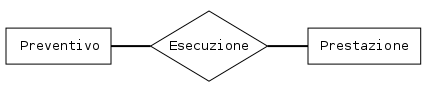
\includegraphics[width=9cm]{images/diagrams/preventivo_prestazione.png}
		\end{figure}
		
		Alla formulazione di ogni preventivo, si fa una stima dei componenti che si reputa saranno necessari per eseguire la prestazione preventivata. Non sempre tale previsione è completamente completamente esatta, generalmente i componenti effettivamente utilizzati in una prestazione sono diversi da quelli previsti in un preventivo.
		L'associazione tra i \emph{Componenti} e il \emph{Preventivo} risulta immediata.
		
		\begin{figure}[H]
			\centering
			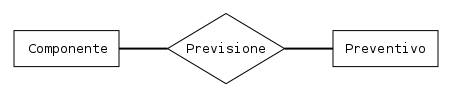
\includegraphics[width=9cm]{images/diagrams/preventivo_componente.png}
		\end{figure}
		
		Prima di esplicitare l'associazione tra le prestazioni eseguite ed i componenti effettivamente utilizzati, affrontiamo la questione degli ordini e del magazzino.
		
		L'acquisto di articoli presso un fornitore è formalizzato in un ordine, il quale, come da specifiche, è organizzato in più forniture, ovvero insiemi di articoli di uno stesso componente.
		Ad un \emph{Ordine} sono associate una o più \emph{Forniture} di articoli, ognuna delle quali fanno riferimento ad un \emph{Componente}.
		
		\begin{figure}[H]
			\centering
			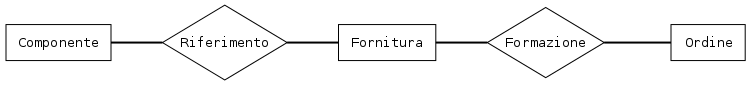
\includegraphics[width=11.5cm]{images/diagrams/componente_ordine.png}
		\end{figure}
		
		Il magazzino, nella realtà, è composto dai vari articoli acquistati che sono in attesa di essere utilizzati. La classificazione degli articoli avviene, in primo luogo per componente, in secondo luogo per fornitura d'appartenenza. Non vi è così il bisogno di registrare ogni articolo individualmente, ma basterà riferirsi alle relative forniture.
		Il \emph{Magazzino} è una composizione di \emph{Forniture} i cui articoli sono depositati in attesa di essere utilizzati.
		
		\begin{figure}[H]
			\centering
			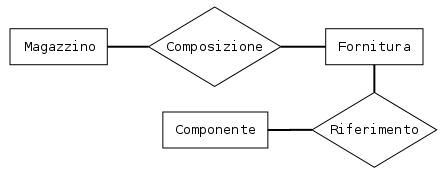
\includegraphics[width=9cm]{images/diagrams/magazzino_fornitura.png}
		\end{figure}
		
		Per identificare con precisione quali articoli sono stati utilizzati per l'esecuzione di una prestazione, sarà sufficiente riferirsi alla fornitura relativa agli stessi. Da questa si ottengono le informazioni sul componente (quindi il prezzo di vendita e il tempo di validità) e sulla data d'acquisto.
		Ad ogni utilizzo, si provvederà ad aggiornare le quantità rimanenti degli articoli delle forniture utilizzate.
		Per l'esecuzione di una \emph{Prestazione} si possono utilizzare gli articoli di più \emph{Forniture}.
		
		\begin{figure}[H]
			\centering
			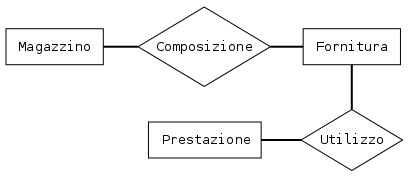
\includegraphics[width=9cm]{images/diagrams/prestazione_fornitura.png}
		\end{figure}
		
		Passiamo alla questione degli operatori. Una prestazione viene eseguita da uno o più operatori. Di ogni operatore si vuole tener traccia dei turni di lavoro effettuati.
		Alla \emph{Prestazione}, saranno associati uno o più \emph{Operatori} ad ognuno dei quali sono associati i relativi \emph{Turni} di lavoro.
		
		\begin{figure}[H]
			\centering
			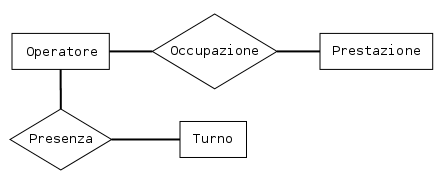
\includegraphics[width=9cm]{images/diagrams/operatore_turno_prestazione.png}
		\end{figure}
		
		Occupiamoci ora delle zone periferiche dello schema. Un preventivo viene effettuato quando un cliente richiede un intervento alla propria auto.
		Ad ogni \emph{Cliente} vengono associate una o più \emph{Autovetture}. Ogni \emph{Preventivo} si riferisce ad una specifica \emph{Autovettura}.
		
		\begin{figure}[H]
			\centering
			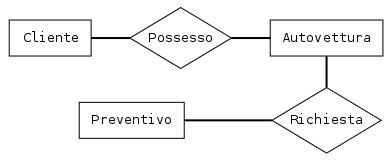
\includegraphics[width=9cm]{images/diagrams/cliente_autovettura_preventivo.png}
		\end{figure}
		
		Ogni \emph{Ordine} viene effettuato presso un \emph{Fornitore}.
		
		\begin{figure}[H]
			\centering
			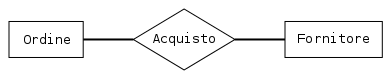
\includegraphics[width=9cm]{images/diagrams/ordine_fornitore.png}
		\end{figure}
		
		Notiamo che \emph{Cliente} rappresenta sia \emph{Privati} che \emph{Aziende} (rispettivamente, clienti non dotati di partita iva e clienti dotati di partita iva).
		
		\begin{figure}[H]
			\centering
			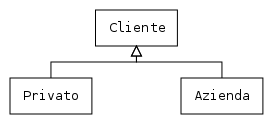
\includegraphics[width=7.5cm]{images/diagrams/cliente.png}
		\end{figure}
		
		Inoltre \emph{Clienti}, \emph{Fornitori} ed \emph{Operatori} possono essere generalizzati dall'entità \emph{Persona}.
		
		\begin{figure}[H]
			\centering
			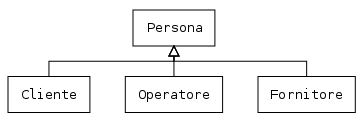
\includegraphics[width=10cm]{images/diagrams/persona.png}
		\end{figure}
		
		Ad ogni \emph{Persona} saranno associati uno o più \emph{Recapiti}.
		
		\begin{figure}[H]
			\centering
			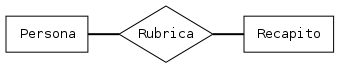
\includegraphics[width=9cm]{images/diagrams/persona_recapito.png}
		\end{figure}
		
		Possiamo concludere lo sviluppo della struttura del diagramma ER affrontando la questione delle transazioni. Avviene una \emph{Transazione} ogni volta che viene versato un acconto per un \emph{Preventivo}, ogni volta che viene saldata la \emph{Fattura} di una \emph{Prestazione}, ogni volta che viene pagato un \emph{Ordine} ed ogni volta che viene pagato lo stipendio di un \emph{Operatore}.
		
		\begin{figure}[H]
			\centering
			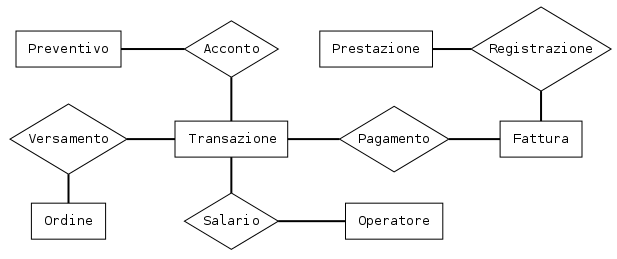
\includegraphics[width=12cm]{images/diagrams/transazione.png}
		\end{figure}
			
		Il diagramma in figura \ref{fig:scheletro_er} rappresenta lo scheletro dello schema ER.
		
		\begin{sidewaysfigure}
			\centering
			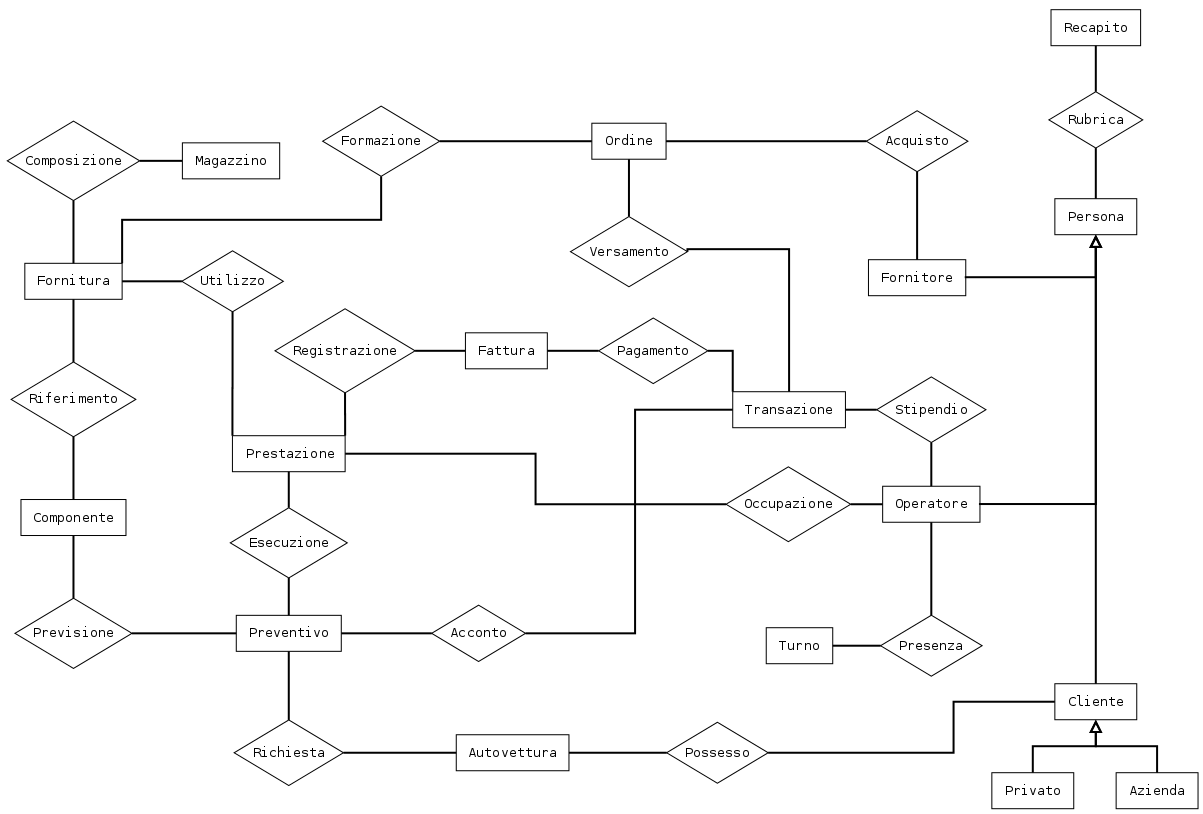
\includegraphics[width=22cm]{images/diagrams/schema.png}
			\caption{Scheletro del diagramma ER}
			\label{fig:scheletro_er}
		\end{sidewaysfigure}
	
	\subsection{Sviluppo delle Componenti dello Schema}
	
		Ottenuto lo scheletro generale del diagramma ER procediamo ad esplicitare, delle entità principali, l'insieme degli attributi che ognuna di esse possiede.
		Una volta sviluppati gli attributi delle entità principali svilupperemo le relationship che le legano, raggruppandole tra loro sulla falsariga dei modelli elaborati allo step precedente.
		
		\begin{description}
			\item[NB]
				Ogni generalizzazione effettuata è da considerarsi totale.
		\end{description}
		
		\subsubsection{Persona}
		
			In figura \ref{fig:persona} troviamo lo sviluppo degli attributi dell'entità \emph{Persona} e delle relative entità che la estendono.
			
			L'identificativo dell'entità \emph{Persona} è costituito dall'attributo "Codice Fiscale o P.Iva", capace di identificare così sia privati che aziende. Ogni \emph{Persona} è caratterizzata anche dall'attributo composto "Indirizzo", sviluppabile in "Città", "Via", "Civico", "CAP", che identifica l'indirizzo di riferimento della persona stessa.
			
			Le entità figlie di \emph{Persona} sono \emph{Fornitore}, \emph{Operatore} e \emph{Cliente}. Quest'ultimo può essere ulteriormente scomposto in altre due entità figlie \emph{Privato} e \emph{Azienda}.
			
			\emph{Privato} possiede gli attributi "Nome", "Cognome" e "Numero Documento Identità", mentre per l'entità \emph{Azienda} si è reso necessario avere solamente l'attributo "Ragione Sociale".
			
			\emph{Fornitore} è dotato degli attributi "Ragione Sociale", "IBAN", "Tempi Consegna" (numero di giorni feriali necessari in media affinchè la merce ordinata al fornitore arrivi) e "Modalità Pagamento" (specifica la modalità di pagamento tra assegno e bonifico bancario).
			
			\emph{Operatore} ha gli attributi "Nome", "Cognome", "IBAN", "Stipendio" (ammontare dello stipendio mensile, se il lavoratore ha un contratto a retribuzione fissa), "Retribuzione oraria" (se il lavoratore ha un contratto che prevede uno stipendio calcolato in base alle ore di lavoro), "Modalità Riscossione" (specifica la modalità di riscossione dello stipendio tra assegno, bonifico o contanti\footnote{Applicabile solo nel caso in cui l'ammontare del pagamento non superi l'importo massimo a norma di legge. Attualmente il limite per i pagamenti in contanti ammonta a 1000.00\EUR.}) e "Dati Anagrafici" (attributo composto da "Data di Nascita", "Comune di Nascita", "Provinicia").
						
			\begin{figure}[H]
				\centering
				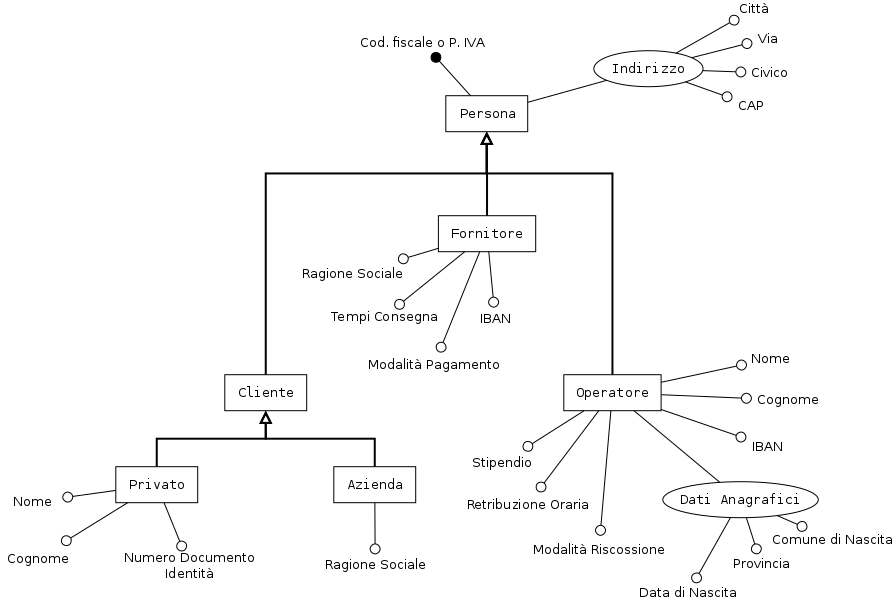
\includegraphics[width=12cm]{images/finitures/persona.png}
				\caption{Sviluppo di Persona}
				\label{fig:persona}
			\end{figure}
		
		\subsubsection{Autovettura}
			
			Continuiamo con gli attributi che caratterizzano l'entità \emph{Autovettura} (Diagramma in figura \ref{fig:autovettura})
			
			\begin{figure}[H]
				\centering
				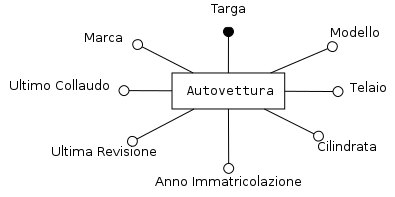
\includegraphics[width=9cm]{images/finitures/autovettura.png}
				\caption{Sviluppo dell'entità Autovettura}
				\label{fig:autovettura}
			\end{figure}
			
			\emph{Autovettura} comprende gli attributi "Targa", "Marca", "Modello", "Telaio" (numero di serie del telaio che identifica univocamente un veicolo che viene inciso sul telaio del veicolo e viene indicato nel libretto di circolazione), "Ultima Revisione" e "Ultimo Collaudo" (rispettivamente le date in cui è stata effettuata la revisione dell'auto e il collaudo di un eventuale impianto di alimentazione differente da quello di fabbricazione), "Anno di Immatricolazione", "Cilindrata".
		
			Si è scelto l'attrubuto "Targa" come chiave primaria dell'entità piuttosto che l'attributo "Telaio" nonostante anche quest'ultimo identifichi univocamente l'autovettura. Riteniamo che sia più agevole identificare un'autovettura attraverso la targa poichè tale informazione è più facilmente reperibile rispetto al seriale del telaio.
			
		\subsubsection{Preventivo}
		
			In figura \ref{fig:preventivo}, il diagramma espone gli attributi dell'entità \emph{Preventivo}.
			
			\emph{Preventivo} è costituito dagli attributi "Codice" (identificativo numerico interno all'azienda del preventivo fornito), "Data Emissione", "Tempo Stimato" (ovvero la stima del numero di giorni necessari all'esecuzione del lavoro), "Data Inizio" (data in cui il lavoro è stato pianificato per essere eseguito), "Categoria" (riparazione, installazione di un impianto a metano, installazione di un impianto a gpl, collaudo o revisione), "Sistema Alimentazione" (attributo necessario per le installazioni di nuovi impianti, necessari a specificare il sistema di alimentazione tra sistema a iniezione e sistema ad aspirazione), "Sintomi" (ovvero una breve descrizione del malfunzionamento riscontrato, nel caso in cui si tratti di una riparazione), "Costo Servizi" (composizione della stima dei costi dei servizi aggiuntivi e della manodopera).
			
			\begin{figure}[H]
				\centering
				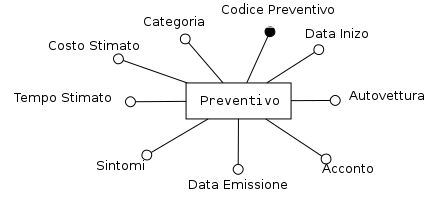
\includegraphics[width=12cm]{images/finitures/preventivo.png}
				\caption{Sviluppo dell'entità Preventivo}
				\label{fig:preventivo}
			\end{figure}
			
		\subsubsection{Prestazione}
			
			Gli attributi dell'entità \emph{Prestazione} vengono esplicitati dal diagramma in figura \ref{fig:prestazione}.
			
			\emph{Prestazione} è composta dagli attributi "Preventivo" (codice identificativo del preventivo di riferimento), "Tempi Esecuzione" (giorni necessari effettivamente all'esecuzione del lavoro preventivato), "Malfunzionamento" (descrizione breve della natura e dell'origine del malfunzionamento riscontrato), "Procedimento" (descrizione concisa ed essenziale del procedimento utilizzato per eliminare i malfunzionamenti), "Costo Servizi" (attributo composto dal costo \emph{effettivo} dei servizi aggiuntivi e della manodopera).
		
			Dovendo tener traccia del preventivo di riferimento a fronte di una prestazione fornita, abbiamo scelto l'attributo \emph{Preventivo} come chiave primaria, dal momento che non vi possono essere più prestazioni a fronte dello stesso preventivo.
		
			\begin{figure}[H]
				\centering
				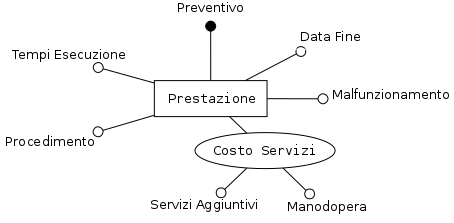
\includegraphics[width=9cm]{images/finitures/prestazione.png}
				\caption{Sviluppo dell'entità Prestazione}
				\label{fig:prestazione}
			\end{figure}
		
		\subsubsection{Componente}
			
			Nel diagramma in figura \ref{fig:componente} troviamo l'entità \emph{Componente} ed i relativi attributi.
			
			L'entità \emph{Componente} comprende gli attributi "Codice" (identificativo numerico interno del componente), "Nome", "Validità" (giorni dalla data di acquisto dopo i quali il componente diventa inutilizzabile), "Quantità Minima" (quantitativo minimo da avere sempre in magazzino), "Prezzo Vendita" (prezzo unitario al quale il componente viene venduto). 
			
			\begin{figure}[H]
				\centering
				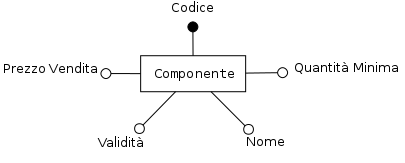
\includegraphics[width=9cm]{images/finitures/componente.png}
				\caption{Sviluppo di Componente}
				\label{fig:componente}
			\end{figure}
		
		\subsubsection{Fattura}
		
			Nel diagramma in figura \ref{fig:fattura}, l'entità \emph{Fattura} ed i suoi attributi.
		
			\begin{figure}[H]
				\centering
				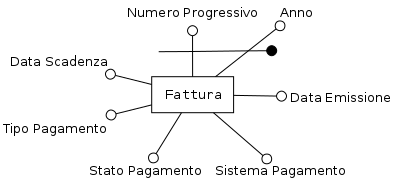
\includegraphics[width=9cm]{images/finitures/fattura.png}
				\caption{Sviluppo di Transazione}
				\label{fig:fattura}
			\end{figure}
			
			\emph{Fattura} è composta dagli attributi "Numero Progressivo" e "Anno" (coppia di attributi identificatori, derivano direttamente dalla struttura reale delle fatture), "Totale" (descrive il prezzo totale della prestazione, è composto da "Imposte" ed "Imponibile"), "Data Emissione", "Sistema Pagamento" (specifica uno dei due sistemi di pagamento accettati: rimessa diretta e rimessa differita), "Tipo Pagamento" (metodologie di pagamento accettate: bonifico, contanti o assegno), "Stato Pagamento" (attributo booleano che permette di distinguere le fatture saldate da quelle non ancora pagate), "Data Scadenza" (data entro la quale la fattura deve essere saldata).
		
		\subsubsection{Transazione}
			
			Il diagramma in figura \ref{fig:transazione} raffigura lo sviluppo degli attributi dell'entità \emph{Transazione}.
			
			L'entità \emph{Transazione} è semplicemente composta dagli attributi "Codice", "Quota" (ammontare della transazione di denaro: quantità positiva per le transazioni entranti, negativa per quelle uscenti), "Data".
						
			\begin{figure}[H]
				\centering
				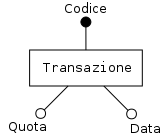
\includegraphics[width=4.5cm]{images/finitures/transazione.png}
				\caption{Sviluppo di Transazione}
				\label{fig:transazione}
			\end{figure}
		
		\subsubsection{Raffinamenti Successivi}
			
			Esplicitati gli attributi delle principali entità, procediamo a legarle tra loro sviluppando le relationship ed alcune entità minori.
			
			Ripercorrendo i passi dello sviluppo dello scheletro del diagramma ER, partiamo dalle relationship che legano le entità \emph{Cliente}, \emph{Autovettura}, \emph{Preventivo} (diagramma in figura \ref{fig:cliente_autovettura_preventivo}).		
		
			\begin{figure}
				\centering
				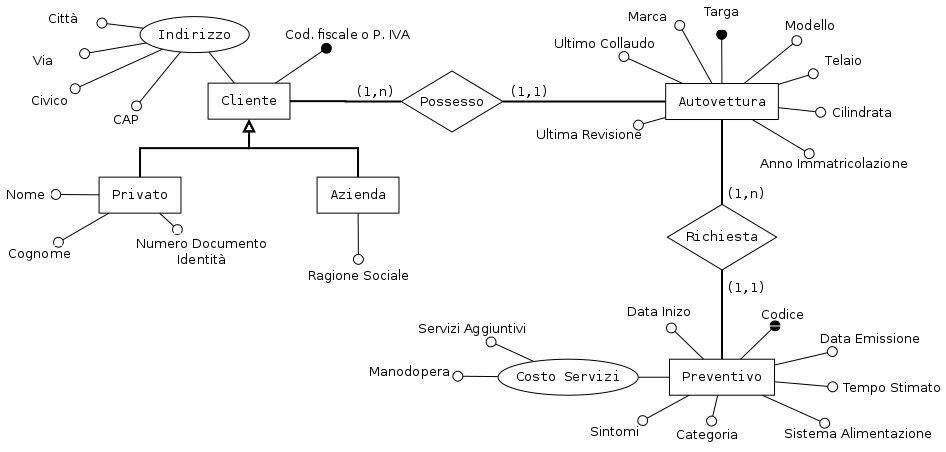
\includegraphics[width=13cm]{images/finitures/cliente_autovettura_preventivo.png}
				\caption{Sviluppo delle relationship che legano Cliente, Autovettura e Preventivo}
				\label{fig:cliente_autovettura_preventivo}
			\end{figure}
			
			Chiaramente ad ogni cliente registrato, saranno associate una o più autovetture di sua propiertà. Ad ogni autovettura saranno associati uno o più preventivi di interventi riferiti all'autovettura stessa (Diagramma in figura \ref{fig:cliente_autovettura_preventivo}).
			
			Se l'intervento preventivato viene realizzato, al preventivo sarà associata una ed una sola prestazione. La stipulazione del preventivo non è vincolante nei confronti del cliente, quindi non è vero che ad ogni preventivo corrisponde una prestazione (Diagramma in figura \ref{fig:preventivo_prestazione}).
			
			\begin{figure}[H]
				\centering
				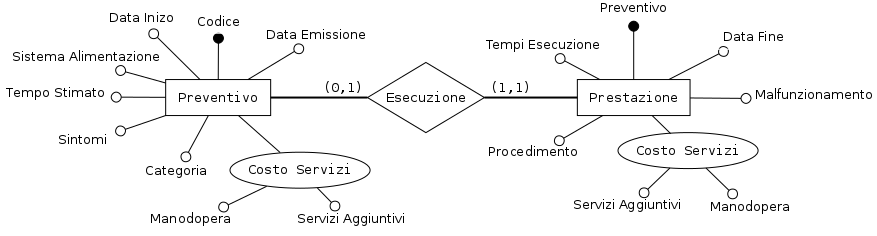
\includegraphics[width=13cm]{images/finitures/preventivo_prestazione.png}
				\caption{Sviluppo della relationship che lega Preventivo e Prestazione}
				\label{fig:preventivo_prestazione}
			\end{figure}
			
			I componenti previsti nelle riparazioni vengono descritti tramite la relazione \emph{Previsione} che lega le entità \emph{Componente} e \emph{Preventivo}. In ogni preventivo si può prevedere di utilizzare nessuno, uno o più componenti. L'utilizzo di uno stesso componente può essere previsto - ovviamente - nella formulazione di più preventivi.
			Si consulti il diagramma in figura \ref{fig:preventivo_componente}.
			
			\begin{figure}[H]
				\centering
				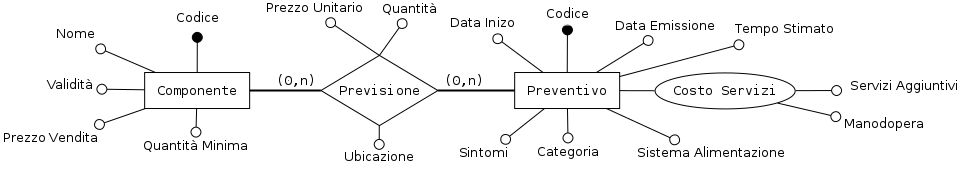
\includegraphics[width=13cm]{images/finitures/preventivo_componente.png}
				\caption{Sviluppo di Preventivo e Componente}
				\label{fig:preventivo_componente}
			\end{figure}
			
			L'attributo "Ubicazione" della relazione \emph{Previsione} rappresenta l'ubicazione dei componenti utilizzati nelle installazioni di nuovi impianti (si consultino anche le specifiche riguardanti i preventivi alla sottosezione "Frasi relative ai Preventivi" \ref{sec:frasi_preventivi}).
			
			Per la registrazione degli articoli acquistati sono state introdotte in fase di sviluppo dello scheletro dello schema ER le entità \emph{Ordine} e \emph{Fornitura}. Tali entità, prese singolarmente, sono poco significative, essendo fortemente legate tra di loro (si faccia riferimento al diagramma in figura \ref{fig:fornitore_ordine_fornitura_componente}).
			
			I contratti di acquisto con i fornitori vengono modellati dall'entità \emph{Ordine}. Naturalmente presso lo stesso fornitore si possono effettuare più ordini, ma un ordine si riferisce ad un singolo fornitore. \emph{Ordine} e \emph{Fornitore} sono legati dalla relationship \emph{Acquisto}.
			
			\begin{figure}[H]
				\centering
				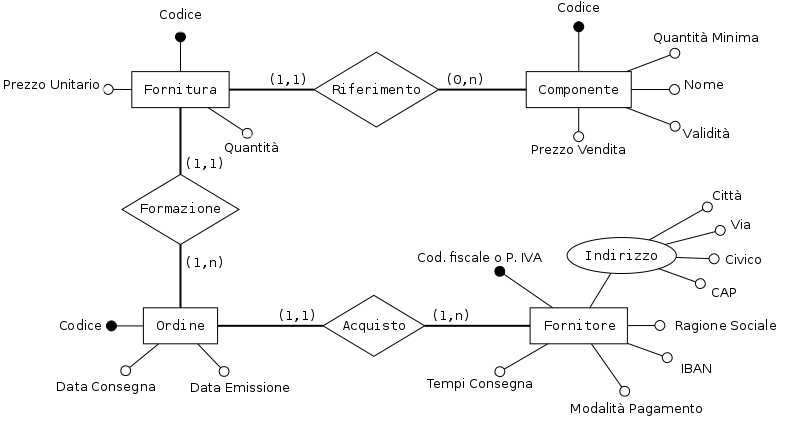
\includegraphics[width=13cm]{images/finitures/fornitore_ordine_fornitura_componente}
				\caption{Sviluppo delle relazioni che legano il Fornitore, l'Ordine d'acquisto, le Forniture e i Componenti}
				\label{fig:fornitore_ordine_fornitura_componente}
			\end{figure}
			
			Ogni ordine è composto da una o più forniture, le quali, a loro volta, sono composte da uno o più articoli dello stesso componente. Ad ogni istanza dell'entità \emph{Fornitura} si associa - tramite la relationship \emph{Riferimento} - una ed una sola istanza dell'entità \emph{Componente}. Di contro, lo stesso componente può essere acquistato in diverse forniture.
			Quindi ogni istanza di \emph{Fornitura} sarà associata ad una ed una sola istanza di \emph{Ordine} tramite la relationship \emph{Formazione}. Un ordine vedrà associate a sè una o più forniture.
			
			\begin{figure}
				\centering
				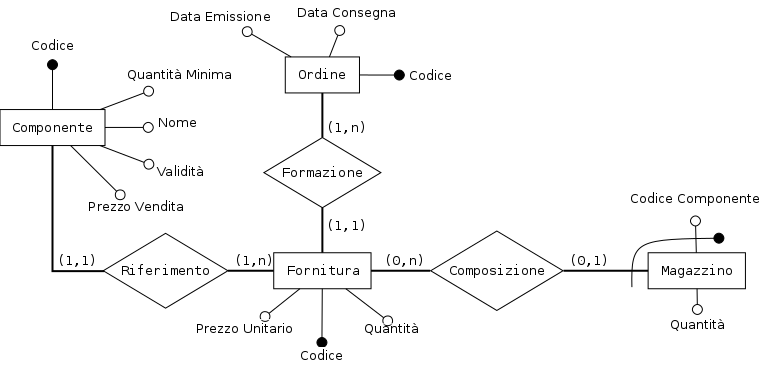
\includegraphics[width=13cm]{images/finitures/componente_fornitura_ordine_magazzino.png}
				\caption{Introduzione del Magazzino}
				\label{fig:componente_fornitura_ordine_magazzino}
			\end{figure}
			
			Un'ulteriore entità da aggiungere a questo gruppo è quella del magazzino. Abbiamo definito \emph{Magazzino} come una raccolta di forniture attive, cioè di forniture i quali articoli sono ancora presenti nel magazzino fisico, pronti per essere utilizzati. Legando \emph{Magazzino} con \emph{Fornitura} si modella tale associazione. La relationship \emph{Composizione} associa ad ogni istanza di \emph{Magazzino} una ed una sola istanza di \emph{Fornitura}. Da notare che il codice della fornitura e il codice del componente di riferimento, formano la chiave primaria di tale entità.
			Fare riferimento al diagramma in figura \ref{fig:componente_fornitura_ordine_magazzino}.
			
			Da notare che l'attributo "Quantità" dell'entità \emph{Magazzino} descrive il numero di articoli di uno specifico componente, acquistati in una certa fornitura, ancora disponibili in magazzino.
			
			All'esecuzione di una prestazione, come da specifiche, è necessario specificare il tipo e la quantità di articoli utilizzati. La prima soluzione che ci è sembrata valida è stata quella di associare, ad ogni istanza dell'entità \emph{Prestazione} le istanze interessate dell'entità \emph{Componente} attraverso la relationship \emph{Utilizzo}. Tale relationship avrebbe avuto l'attributo "Quantità", necessario per specificare la quantità degli articoli utilizzati per ogni componente.
			
			Tuttavia, tale design si è rivelato non adeguato a soddisfare tutte le specifiche. Il problema più evidente risiedeva nel fatto che, essendo le istanze dell'entità \emph{Componente} composte da informazioni descrittive, pressocchè invarianti (eccezion fatta per quanto riguarda il "Prezzo di Vendita"), non vi è il modo per risalire al preciso articolo fisico utilizzato nella riparazione\footnote{Non potendo risalire al preciso articolo utilizzato, non si ha a disposizione la data di acquisto, quindi viene meno la realizzabilità del meccanismo che permette di utilizzare per primi gli articoli dei componenti la cui data di scadenza è più vicina di altri.}.
			
			All'entità \emph{Prestazione} vengono quindi associate zero, una o più istanze dell'entità \emph{Fornitura}, avendo così a disposizione sia le informazioni che descrivono genericamente il componente, sia quelle che caratterizzano con precisione l'articolo utilizzato nella prestazione. 

			\begin{figure}
				\centering
				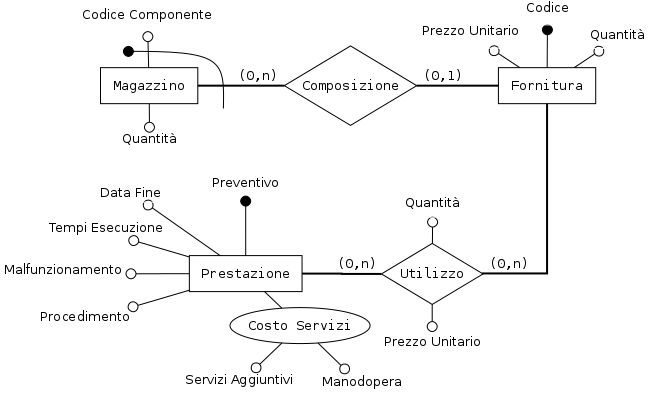
\includegraphics[width=11.5cm]{images/finitures/prestazione_fornitura.png}
				\caption{Utilizzo di componenti un una prestazione}
				\label{fig:ordine_fornitore}
			\end{figure}
			
			L'attributo "Quantità" della relationship \emph{Utilizzo} non necessita di ulteriori spiegazioni, mentre l'attributo "Prezzo Unitario" si rende necessario, in quanto il prezzo di vendita di un componente, ragionevolmente, varia nel tempo.
			
			Ad esecuzione ultimata di una prestazione avviene la registrazione della fattura. Ad ogni istanza dell'entità \emph{Prestazione} sarà associata, tramite la relationship \emph{Registrazione} obbligatoriamente una ed una sola istanza dell'entità \emph{Fattura}. 		
			
			Le istanze dell'entità \emph{Fattura} vengono identificate dalla coppia di attributi "Numero Progressivo" ed "Anno", così come avviene nella realtà di interesse\footnote{Le fatture vengono identificate dall'anno di emissione e dal numero progressivo. Ogni anno tale numero viene azzerato.}.
			
			\begin{figure}[H]
				\centering
				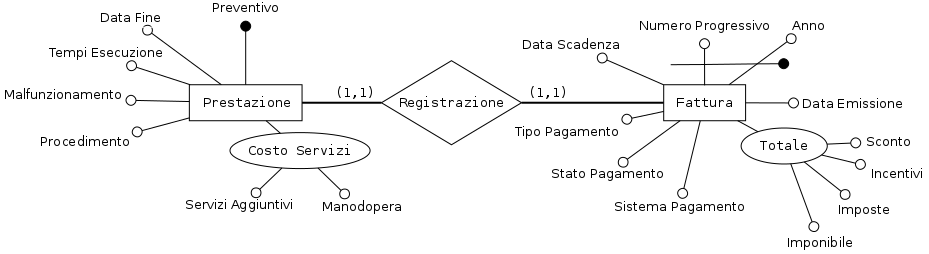
\includegraphics[width=11.5cm]{images/finitures/prestazione_fattura.png}
				\caption{Sviluppo della relationship tra Prestazione e Fattura}
				\label{fig:prestazione_fattura}
			\end{figure}
			
			Gli sviluppi dei diagrammi introdotti fin'ora permettono di affrontare il legame di \emph{Transazione} con le altre entità. A quest'ultima si possono associare istanze di tutte le entità che modellano dati di porzioni di processo che prevedono il verificarsi di transazioni monetarie. Alla stipulazione di un preventivo può essere richiesto il versamento di un acconto, alla consegna gli ordine sarà necessario effettuare una versamento al fornitore, mensilmente bisognerà registrare gli stipendi versati agli operatori e quando una fattura viene saldata bisognerà registrare tale transazione di denaro.
			
			\begin{figure}
				\centering
				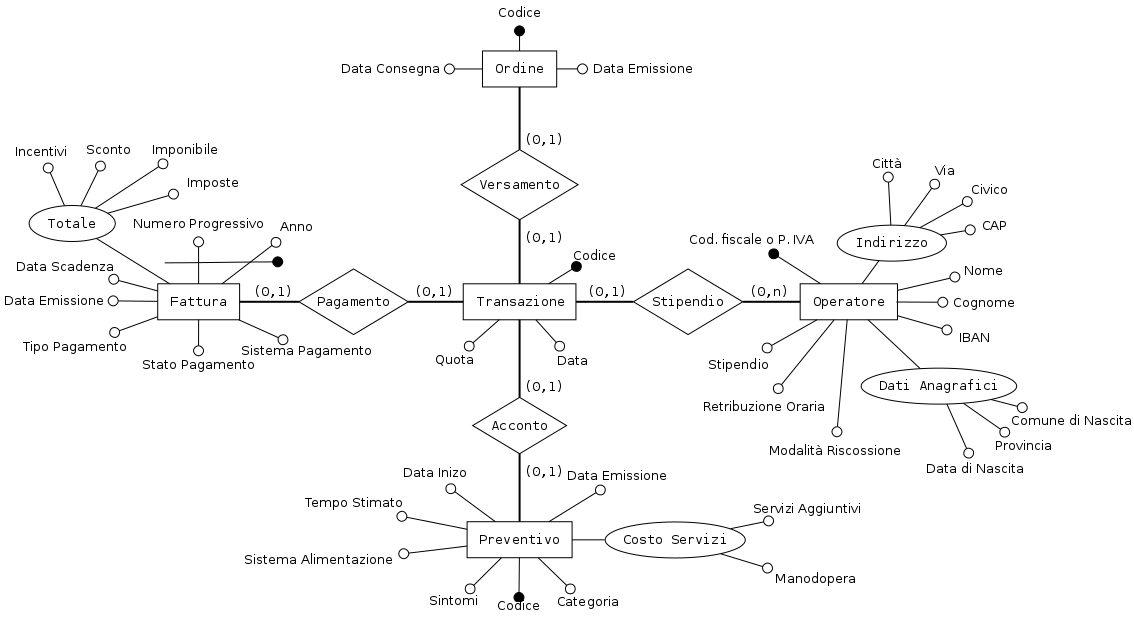
\includegraphics[width=13cm]{images/finitures/transazione_fattura_preventivo_operatore_ordine.png}
				\caption{Sviluppo delle relationship con cui Transazione si lega alle altre entità}
				\label{fig:transazione_fattura_preventivo_operatore_ordine}
			\end{figure}
			
			Nel diagramma in figura \ref{fig:transazione_fattura_preventivo_operatore_ordine} vi è la rappresentazione di come le entità \emph{Preventivo}, \emph{Ordine}, \emph{Operatore}, \emph{Fattura} vengono associate a \emph{Transazione}.
			
			Esaminiamo le ultime componenti del diagramma ER che non sono state ancora analizzate.
			
			In figura \ref{fig:operatore_prestazione} il diagramma descrive la relationship \emph{Occupazione} che associa le istanze di \emph{Prestazione} a quelle di \emph{Operatore}. Ad ogni istanza di \emph{Prestazione} infatti devono essere associate una o più instanze di \emph{Operatore}, in modo da tener traccia dei dipendenti che sono stati impiegati nell'esecuzione della prestazione ad un'autovettura. Ovviamente la stessa istanza di \emph{Operatore} può essere associata a più istanze di \emph{Prestazione}.
			
			\begin{figure}
				\centering
				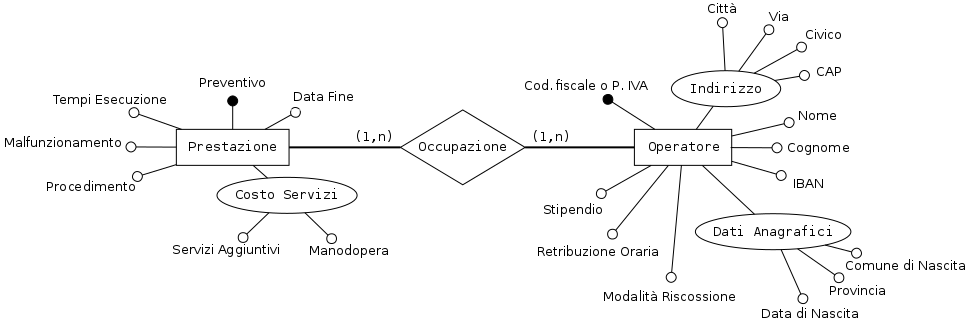
\includegraphics[width=11.5cm]{images/finitures/operatore_prestazione.png}
				\caption{Sviluppo della relationship tra Prestazione e Operatore}
				\label{fig:operatore_prestazione}
			\end{figure}
			
			Riguardo gli operatori è necessario, come da specifiche, registrarne le presenze e gli orari di lavoro. L'entità \emph{Turno}, legata ad \emph{Operatore} tramite la relationship \emph{Presenza} (diagramma in figura \ref{fig:operatore_turno}), assolve tale funzione.
			
			\begin{figure}
				\centering
				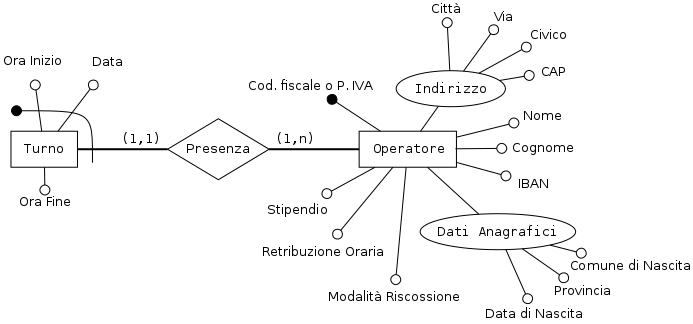
\includegraphics[width=11.5cm]{images/finitures/operatore_turno.png}
				\caption{Turni degli Operatori}
				\label{fig:operatore_turno}
			\end{figure}
			
			L'ultimo punto da sviluppare consiste nella gestione dei recapiti, di qualunque natura essi siano. L'entità \emph{Recapito} è costituita dagli attributi "Recapito" (che è anche chiave primaria) e dall'attributo "Tipo" (consultare le Regole Aziendali alla sezione \ref{sec:business_rules} per i valori che tale attributo può assumere).
			Ad ogni istanza di \emph{Persona} devono essere associati una o più istanze di \emph{Recapito}.
			
			\begin{figure}
				\centering
				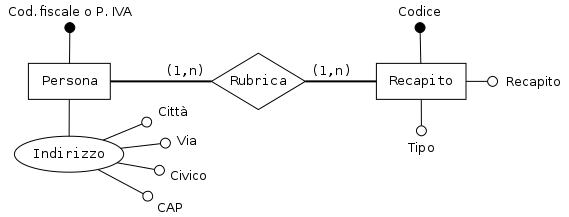
\includegraphics[width=11.5cm]{images/finitures/persona_rubrica.png}
				\caption{Turni degli Operatori}
				\label{fig:persona_recapito}
			\end{figure}
	
	% Diagramma definitivo
	\subsection{Diagramma Entity-Relationship}
		
		L'intero diagramma ER si può trovare in figura \ref{fig:er}.
			
		\begin{sidewaysfigure}
			\centering
			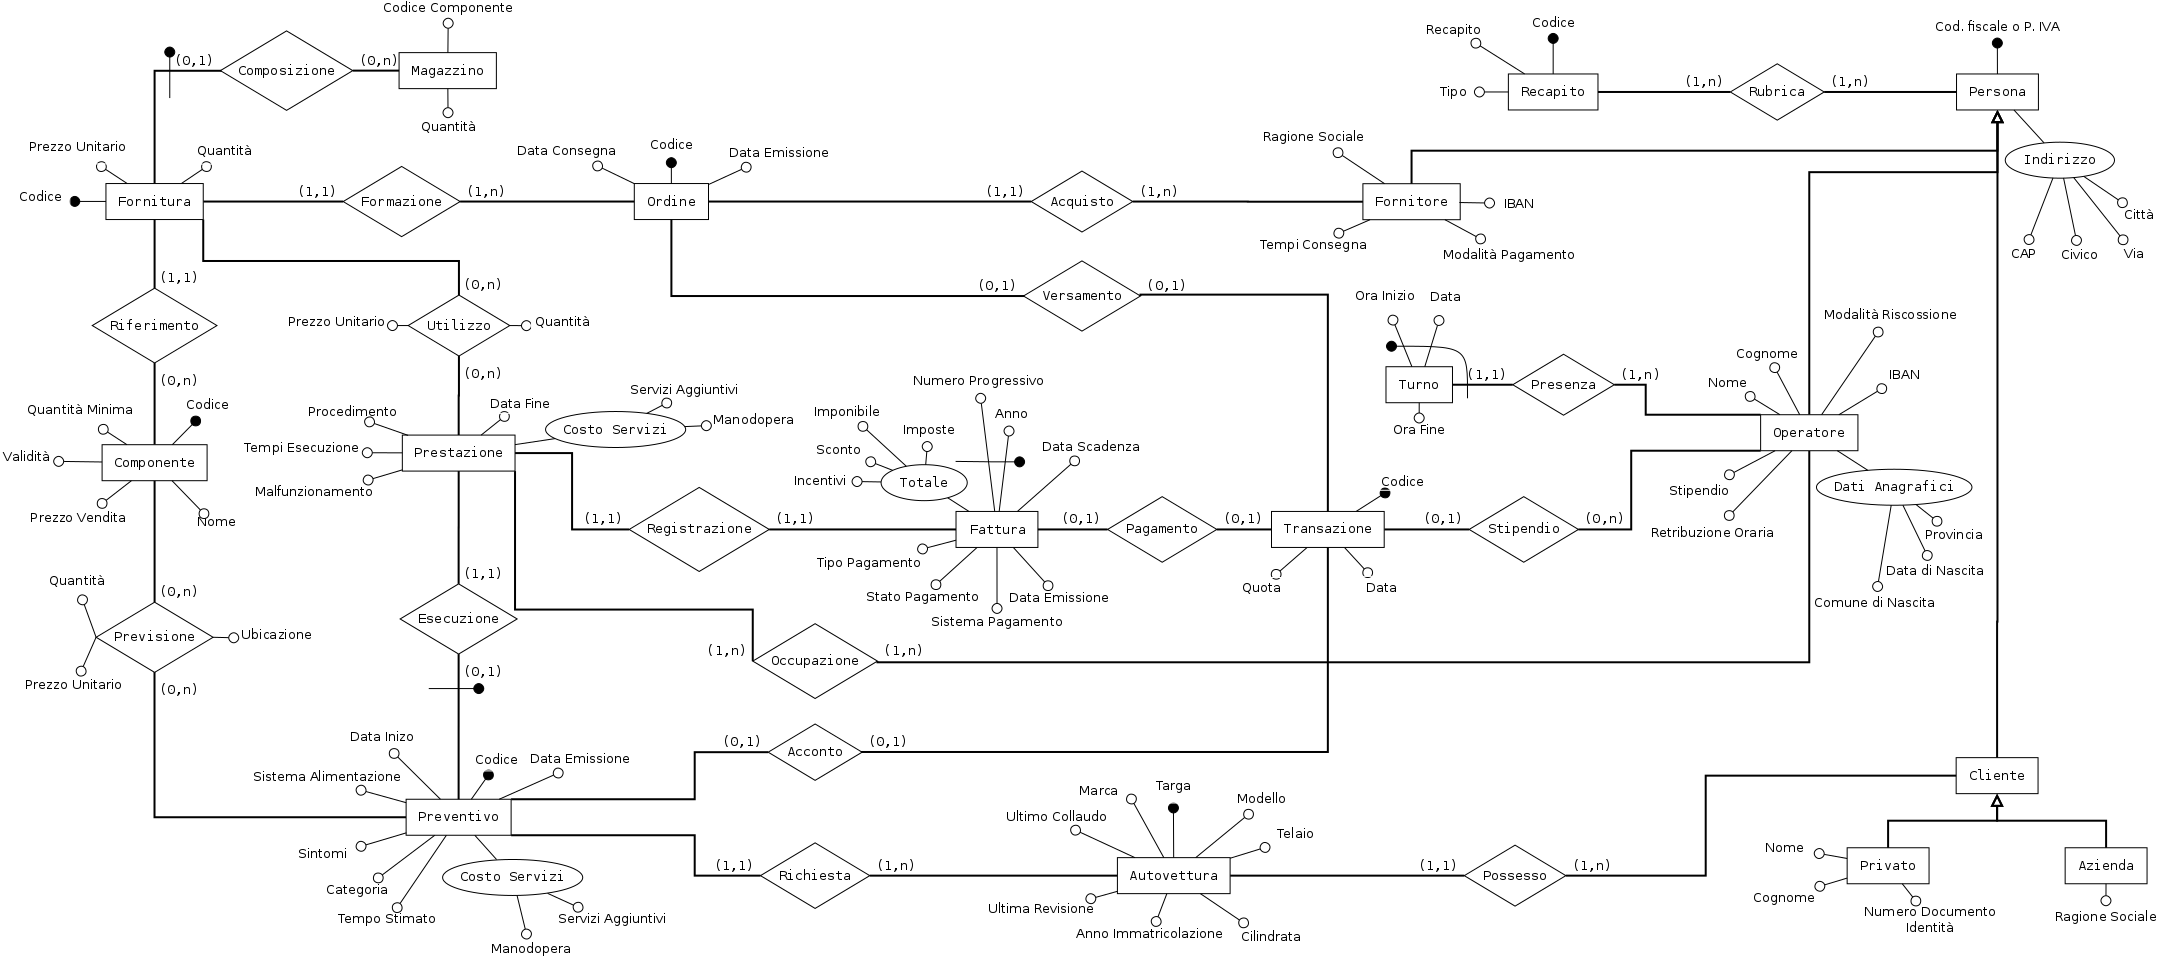
\includegraphics[width=22cm]{images/finitures/schema.png}
			\caption{Scheletro del diagramma ER}
			\label{fig:er}
		\end{sidewaysfigure}

	\subsection{Analisi Qualitativa dello Schema ER}
	
	% Sezione documentativa della progettazione concettuale
	\subsection{Dizionario dei Dati}
	\label{sec:data_dict}
		
		\subsubsection{Entità}
		\label{sec:entities}
			
			{\small
			\begin{longtable}{| p{2cm} | p{4cm} | p{4cm} | p{2cm} |}
				
				\hline
				\textbf{Nome} & 
				\textbf{Descrizione} & 
				\textbf{Attributi} & 
				\textbf{Identificatore} \\ 
				\hline
				
				\endfirsthead
				
				\hline
				\textbf{Nome} & 
				\textbf{Descrizione} & 
				\textbf{Attributi} & 
				\textbf{Identificatore} \\ 
				\hline
				
				\endhead
				
				Persona &
				Soggetto generico che intrattenga rapporti di ogni tipo con l'azienda. &
				Codice Fiscale o P.IVA (Stringa), Città (Stringa), Via (Stringa), Civico (Numerico), CAP (Numerico) &
				Codice Fiscale o P.IVA (Stringa)
				\\ \hline

				Cliente &
				Soggetto che necessita di un servizio da parte dell'azienda. &
				// &
				//
				\\ \hline

				Privato &
				Cliente non dotato di partita IVA. &
				Attributi di Persona, Nome (Stringa), Cognome (Stringa), Numero Documento Identità (Stringa) &
				//
				\\ \hline

				Azienda  &
				Cliente dotato di partita IVA. &
				Attributi di Persona, Ragione Sociale (Stringa) &
				//
				\\ \hline

				Fornitore &
				Azienda che abbia fornito all’officina qualsiasi tipo di componente necessario. &
				Attributi di Persona, Ragione Sociale (Stringa), Tempi Consegna (Numerico), Modalità Pagamento (Stringa), IBAN (Stringa) &
				//
				\\ \hline

				Operatore &
				Lavoratore dell'azienda. &
				Attributi di Persona, Nome (Stringa), Cognome (Stringa), IBAN (Stringa), Stipendio (Numerico), Retribuzione Oraria (Numerico), Modalità Riscossione (Stringa), Comune Nascita (Stringa), Provincia (Stringa), Data Nascita (Data) &
				//
				\\ \hline

				Autovettura &
				Automobile di un cliente che debba subire o abbia già subito un intervento da parte dei lavoratori dell’azienda. &
				Targa (Stringa), Modello (Stringa), Telaio (Stringa), Cilindrata (Numerico), Anno Immatricolazione (Numerico), Ultima Revisione (Data), Ultimo Collaudo (Data), Marca (Stringa) &
				Targa (Stringa)
				\\ \hline

				Preventivo &
				Stima dei costi, dei tempi e dei componenti necessari relativi all’esecuzione di un intervento su un’autovettura. &
				Preventivo (Numerico), Data Emissione (Data), Data Inizio (Data), Categoria (Stringa), Servizi Aggiuntivi (Numerico), Manodopera (Numerico), Tempo Stimato (Numerico), Sintomi (Stringa), Sistema Alimentazione (Stringa) &
				Preventivo (Numerico)
				\\ \hline

				Componente &
				Qualsiasi oggetto fisico necessario alla corretta esecuzione di una riparazione o di una installazione di un impianto su di un’autovettura.  &
				Codice (Numerico), Quantità Minima (Numerico), Prezzo Vendita (Numerico), Validità (Numerico), Nome (Stringa) &
				Codice (Numerico)
				\\ \hline

				Fornitura &
				Insieme dello stesso componente inviata da un fornitore. &
				Codice (Numerico), Prezzo Unitario (Numerico), Quantità (Numerico) &
				Codice (Numerico)
				\\ \hline

				Ordine &
				Insieme di forniture inviate nello stesso momento e dallo stesso ordine. &
				Codice (Numerico), Data Consegna (Data), Data Emissione (Data) &
				Codice (Numerico)
				\\ \hline
				
				Magazzino  &
				Insieme di tutte le forniture non esaurite. &
				Codice Componente (Numerico), Quantità (Numerico) &
				Codice Componente (Numerico), Codice (di \emph{Fornitura})
				\\ \hline

				Prestazione &
				Attività eseguita dagli operatori dell’officina su di un’autovettura. &
				Preventivo (Numerico), Tempi Esecuzione (Numerico), Data Fine (Data), Manodopera (Numerico), Servizi Aggiuntivi (Numerico), Malfunzionamento (Stringa), Procedimento (Stringa) &
				Codice (Numerico)
				\\ \hline

				Turno &
				Arco temporale specifico in cui gli operatori compiono le loro mansioni. &
				Ora Inizio (Numerico), Ora fine (Numerico), Data (Data) &
				Ora Inizio (Numerico), Data (Data), Codice Fiscale o P.IVA (di \emph{Operatore})
				\\ \hline

				Transazione &
				Flusso di denaro uscente o entrante nella cassa dell’attività. &
				Codice (Numerico), Quota (Numerico), Data (Data) &
				Codice (Numerico)
				\\ \hline

				Fattura &
				Documento fiscale relativo ad un pagamento da ricevere da parte di un cliente. &
				Numero Progressivo (Numerico), Anno (Numerico), Data Emissione (Data), Imponibile (Numerico), Imposte (Numerico), Sistema Pagamento (Stringa), Tipo Pagamento (Stringa), Stato Pagamento (Stringa), Data Scadenza (Data) &
				Numero Progressivo (Numerico), Anno (Numerico)
				\\ \hline
				
				Recapito &
				Numero telefonico, indirizzo email o sito web. Qualsiasi recapito telematico utile a contattare una Persona. &
				Recapito (Stringa), Tipo(Stringa) &
				Recapito (Stringa)
				\\ \hline
				
			\end{longtable}
			}

		\subsubsection{Relazioni}
		\label{sec:relationships}
			{\small
			\begin{longtable}{| p{2cm} | p{4cm} | p{4cm} | p{2cm} |}
				
				\hline
				\textbf{Nome} & 
				\textbf{Descrizione} & 
				\textbf{Entità Coinvolte} & 
				\textbf{Attributi} \\ 
				\hline
				
				\endfirsthead
				
				\hline
				\textbf{Nome} & 
				\textbf{Descrizione} & 
				\textbf{Entità Coinvolte} & 
				\textbf{Attributi} \\ 
				\hline
				
				\endhead
				
				Esecuzione &
				Associa ad un Preventivo una Prestazione &
				Preventivo (0, 1) Prestazione (1, 1) &

				\\ \hline

				Previsione &
				Associa i Componenti previsti in fase di stipulazione dei Preventivi &
				Componente (0, N) Preventivo (0, N) &
				Quantità (Numerico) indica la quantità del componente che si prevede di utilizzare
				\\ \hline

				Formazione &
				Associa le forniture che compongono un ordine &
				Fornitura (1, 1) Ordine (1, N) &

				\\ \hline

				Composizione &
				Associa le Forniture che compongono il Magazzino aziendale &
				Magazzino (1, 1) Fornitura (0, 1) &

				\\ \hline

				Riferimento &
				Associa i Componenti che descrivono una Fornitura &
				Componente (1, 1) Fornitura (1, N) &

				\\ \hline

				Utilizzo &
				Associa i Componenti relativi ad un Fornitura effettivamente usati per compiere una prestazione &
				Fornitura (0, N) Prestazione (0, N) &
				Quantità (Numerico) indica la quantità del componente che si è utilizzata\\ \hline

				Occupazione &
				Associa un Operatore ad una Prestazione da svolgere &
				Operatore (0, 1) Prestazione (0, N) &
				\\ \hline

				Presenza &
				Associa un Operatore con il Turno di lavoro effettuato &
				Operatore (1, 1) Turno (0, N) &
				\\ \hline

				Possesso &
				Associa una o più Autovetture ad un Cliente &
				Cliente (1, 1) Autovettura (1, N) &
				\\ \hline

				Richiesta &
				Associa un Preventivo riferito ad una Prestazione da richiedere su una determinata Autovettura &
				Autovettura (0, 1) Preventivo (0, N) &
				\\ \hline

				Acquisto &
				Associa un Ordine effettuato da un determinato Fornitore &
				Ordine (0, N) Fornitore (1, 1) &
				\\ \hline

				Rubrica &
				Associa una generica Persona ai sui Recapiti &
				Persona (0, N) Recapito (1, N) &
				\\ \hline

				Acconto  &
				Associa un Preventivo e la Transazione monetaria che un cliente può lasciare &
				Preventivo (0, 1) Transazione (0, 1) &
				\\ \hline

				Registrazione  &
				Associa una Prestazione ad una Fattura  &
				Prestazione (1, 1) Fattura (1, 1) &
				\\ \hline

				Pagamento &
				Associa il manifestarsi della Transazione di pagamento riferita ad una Fattura &
				Fattura (1, 1) Transazione (0, N) &
				\\ \hline

				Versamento &
				Associa la Transazione monetaria relativa ad un Ordine &
				Ordine (1, 1) Transazione (0, 1) &
				\\ \hline

				Stipendio &
				Associa la Transazione relativa al pagamento dello stipendio di un Operatore &
				Operatore (1, 1) Transazione (0, 1) &
				\\ \hline

			\end{longtable}
			}
		
	
	\subsection{Regole Aziendali}
	\label{sec:business_rules}
	
		\subsubsection{Regole di Vincolo}
		\subsubsection{Regole di Derivazione}

\newpage

% Sezione sulla progettazione logica
%!TEX root = Progetto.tex
\section{Progettazione Logica}
	\subsection{Tavola dei Volumi}
		\subsubsection{Tavola dei Volumi}
		\label{sec:volume_table}

			I volumi delle entità e delle relazioni sono stati stimati facendo riferimento ad un ciclo di vita della base di dati di circa 3 anni. In tale calcolo abbiamo considerato che alcune entità sono soggette ad una iniziale migrazione di dati (come ad esempio l'entità \emph{Fornitore} o \emph{Componente}).
		
			\begin{longtable}{| p{4cm} | p{4cm} | p{4cm} |}


				\hline
				\textbf{Concetto} & 
				\textbf{Tipo} & 
				\textbf{Volume} \\
				\hline
				
				\endfirsthead
				
				\hline
				\textbf{Concetto} & 
				\textbf{Tipo} & 
				\textbf{Volume} \\
				\hline
				\endhead
				
				Persona       & E & 495  \\ \hline
				Cliente       & E & 450  \\ \hline
				Privato       & E & 300  \\ \hline
				Azienda       & E & 150  \\ \hline
				Fornitore     & E & 42   \\ \hline
				Operatore     & E & 3    \\ \hline
				Autovettura   & E & 585  \\ \hline
				Preventivo    & E & 1500 \\ \hline
				Componente    & E & 472  \\ \hline
				Fornitura     & E & 1500 \\ \hline
				Ordine        & E & 300  \\ \hline
				Magazzino     & E & 189  \\ \hline
				Prestazione   & E & 1425 \\ \hline
				Turno         & E & 3000 \\ \hline
				Transazione   & E & 3747 \\ \hline
				Fattura       & E & 1425 \\ \hline
				Recapito      & E & 1077 \\ \hline
				Esecuzione    & R & 1425 \\ \hline
				Previsione    & R & 9000 \\ \hline
				Riferimento   & R & 1500 \\ \hline
				Formazione    & R & 1500 \\ \hline
				Composizione  & R & 472  \\ \hline
				Utilizzo      & R & 8550 \\ \hline
				Occupazione   & R & 2850 \\ \hline
				Presenza      & R & 3000 \\ \hline
				Possesso      & R & 585  \\ \hline
				Richiesta     & R & 1500 \\ \hline
				Acquisto      & R & 300  \\ \hline
				Rubrica       & R & 1077 \\ \hline
				Acconto       & R & 750  \\ \hline
				Registrazione & R & 1425 \\ \hline
				Pagamento     & R & 1425 \\ \hline
				Versamento    & R & 300  \\ \hline
				Salario       & R & 72   \\ \hline
				
			\end{longtable}
			
		\subsubsection{Tavola delle Operazioni}
		
			\begin{longtable}{| p{6.2cm} | p{6.2cm} |}

				\hline
				\textbf{Operazione} & 
				\textbf{Frequenza} \\
				\hline
				
				\endfirsthead
				
				\hline
				\textbf{Operazione} & 
				\textbf{Frequenza} \\
				\hline
				
				\endhead
				
				% Inserimenti
				\ref{op:new_cliente} & 3 volte a settimana \\ \hline
				\ref{op:new_privato} & 2 volte a settimana \\ \hline
				\ref{op:new_azienda} & 1 volta a settimana \\ \hline
				\ref{op:new_auto} & 3 volte a settimana \\ \hline
				\ref{op:new_fornitore} & 4 volte l'anno \\ \hline
				\ref{op:new_componente} & 2 volte al mese \\ \hline
				\ref{op:new_ordine} & 2 volte a settimana \\ \hline
				\ref{op:new_fornitura} & 10 volte a settimana \\ \hline
				\ref{op:new_preventivo} & 10 volte a settimana \\ \hline
				\ref{op:new_prestazione} & 10 volte a settimana \\ \hline
				\ref{op:new_fattura} & 10 volte a settimana \\ \hline
				\ref{op:new_operatore} & 1 volta all'anno \\ \hline
				\ref{op:new_recapito} & 80 volte ogni 3 mesi \\ \hline
				\ref{op:new_presenza} & 2 volte al giorno per ogni operatore \\ \hline
				\ref{op:new_transazione} & 18 volte a settimana \\ \hline

				% Assegnazioni
				\ref{op:ass_componente_preventivo} & 60 volte a settimana \\ \hline
				\ref{op:ass_componente_prestazione} & 60 volte a settimana \\ \hline
				\ref{op:ass_fornitura_ordine} & 10 volte a settimana \\ \hline
				\ref{op:ass_fornitura_magazzino} & 10 volte a settimana \\ \hline

				% Aggiornamenti
				\ref{op:edit_cliente} & 30 volte l'anno \\ \hline
				\ref{op:edit_fornitore} & 2 volte l'anno \\ \hline
				\ref{op:edit_operatore} & 1 volta l'anno \\ \hline
				\ref{op:edit_componente} & 5 volte al mese \\ \hline
				\ref{op:reg_ordine} & 2 volte a settimana \\ \hline

				% Consultazioni
				\ref{op:show_collaudo} & 1 volta a settimana \\ \hline
				\ref{op:show_revisione} & 1 volta a settimana \\ \hline
				\ref{op:show_fattura} & 10 volte a settimana \\ \hline
				\ref{op:show_transazioni} & 1 volta a settimana \\ \hline
				\ref{op:show_riparazioni} & 2 volte al giorno \\ \hline
				\ref{op:show_preventivi} & 2 volte al giorno \\ \hline
				\ref{op:check_componente} & 4 volte al giorno \\ \hline
				\ref{op:check_turni} & 1 volta al mese \\ \hline
				\ref{op:list_componenti} & 1 volta a settimana \\ \hline
				\ref{op:stats_componenti} & 2 volte al mese \\ \hline
				\ref{op:tobuy_componenti} & 1 volta a settimana \\ \hline
				\ref{op:show_recapiti_cliente} & 10 volte a settimana \\ \hline
				\ref{op:show_recapiti_fornitore} & 2 volte a settimana \\ \hline
				\ref{op:show_recapiti_operatore} & 1 volta a settimana \\ \hline
				\ref{op:list_fatture_pending} & 1 volta al giorno \\ \hline
				\ref{op:list_ordini_pending} & 1 volta a settimana \\ \hline
				\ref{op:todo_list} & 1 volta al giorno \\ \hline
				\ref{op:calc_stipendio_operatore} & 1 volta al mese per ogni operatore \\\hline
				\ref{op:stats_prevetivi_prestazioni} & 1 volta a settimana \\ \hline
				\ref{op:stats_costi} & 1 volta a settimana \\ \hline

			\end{longtable}
			
	\subsection{Ristrutturazione dello Schema Concettuale}

		\subsubsection{Analisi delle Derivazioni e della Ridondanza}

			Il modello elaborato nella precedente fase di sviluppo non rispondeva al criterio di minimalità. Gli attributi \emph{Imponibile} e \emph{Imposte} relativi all'entità \emph{Fattura} sono infatti attributi derivabili (Prendere in visione le Regole di Derivazione \ref{rd:imponibile} e \ref{rd:imposte}).

			Giunti ora all'ultima fase progettuale prima dell'effettiva implementazione della base di dati, ci occuperemo di valutare se eliminare o mantenere tale ridondanza, al fine da minimizzare i costi computazionali ed il numero di accessi. Inoltre valuteremo anche l'introduzione di ridondanze non presenti in precedenza, nel caso in cui tale introduzione apportasse sensibili miglioramenti alle prestazioni.

			Le stime degli accessi in lettura/scrittura verranno calcolate in riferimento ad un arco temporale pari ad un mese.

			Le operazioni legate agli attributi ridondanti \emph{Imponibile} ed \emph{Imposte} sono: \ref{op:new_fattura}, \ref{op:new_transazione}, \ref{op:show_fattura}).

			Abbiamo rintracciato altri dati derivabili utilizzati sistematicamente nelle nostre operazioni:

			\setenumerate[1]{label=\arabic*:}
			\begin{enumerate}

				\item \emph{Imponibile} relativo agli ordini effettuati presso i fornitori (\ref{op:new_ordine}\footnote{L'aggiunta di un nuovo ordine prevedere l'inserimento di nuove forniture. Nel calcolo degli accessi, calcoleremo anche questi ultimi}, \ref{op:new_transazione}));
			
				\item \emph{Quantità Presente} dei componenti in magazzino (\ref{op:reg_ordine}, \ref{op:check_componente}, \ref{op:list_componenti}, \ref{op:tobuy_componenti});
			
				\item \emph{Costo Componenti} relativo a \emph{Preventivo} (\ref{op:new_preventivo}, \ref{op:show_preventivi})
			
			\end{enumerate}

			\paragraph{\emph{Imponibile} in Fattura}

				L'\emph{Imponibile} di una fattura può essere ogni volta calcolato basandosi sui valori degli attributi:
				\setenumerate[1]{label=\arabic*)}
				\begin{enumerate}
					\item \emph{Quantità} ($q_i$) e \emph{Prezzo Unitario} ($p_i$) della relationship \emph{Utilizzo} che lega l'istanza della \emph{Prestazione} cui la fattura fa riferimento all'i-esima istanza di \emph{Fornitura}, in riferimento ai componenti utilizzati nella prestazione;
					\item \emph{Servizi Aggiuntivi} ($C_s$) e \emph{Manodopera} ($C_m$) relativi all'entità \emph{Prestazione};
					\item \emph{Sconto} ($S$), relativo all'entità \emph{Fattura}.
				\end{enumerate}

				$$ Imponibile = \left( C_s + C_m + \sum_{i=1}^n p_i q_i \right)\left(1 - \frac{S}{100}\right) $$

				Valutiamo la possibilità eliminare l'attributo ridondante \emph{Imponibile}.

				\subparagraph{Assenza di Ridondanza}
					Analizziamo il numero di accessi ipotizzando di non avere a disposizione l'attributo \emph{Imponibile} per l'entità \emph{Fattura}.

					\vspace{2ex}
					% Nuova fattura, no ridondanza
					\begin{tabular}{| p{3cm} | p{3cm} | p{3cm} | p{3cm} |}
						\hline
						\multicolumn{4}{|c|}{\textbf{\ref{op:new_fattura}}} \\ \hline
						\textbf{Concetto} & \textbf{Costrutto} & \textbf{Accessi} & \textbf{Tipo} \\ \hline
						Fattura & E & 1 & L \\
						Fattura & E & 1 & S \\
						\hline
					\end{tabular}

					% Nuova transazione, no ridondanza
					\begin{tabular}{| p{3cm} | p{3cm} | p{3cm} | p{3cm} |}
						\hline
						\multicolumn{4}{|c|}{\textbf{\ref{op:new_transazione}}} \\ \hline
						\textbf{Concetto} & \textbf{Costrutto} & \textbf{Accessi} & \textbf{Tipo} \\ \hline
						Fattura 		& E & 1 & L \\
						Prestazione 	& E & 1 & L \\
						Utilizzo 		& R & 6 & L \\
						Transazione 	& E & 1 & S \\
						\hline
					\end{tabular}

					% Dati per la stampa di fatture, no ridondanza
					\begin{tabular}{| p{3cm} | p{3cm} | p{3cm} | p{3cm} |}
						\hline
						\multicolumn{4}{|c|}{\textbf{\ref{op:show_fattura}}} \\ \hline
						\textbf{Concetto} & \textbf{Costrutto} & \textbf{Accessi} & \textbf{Tipo} \\ \hline
						Fattura 	& E & 1 & L \\
						Prestazione & E & 1 & L \\
						Utilizzo 	& R & 6 & L \\
						Preventivo 	& E & 1 & L \\
						Autovettura & E & 1 & L \\
						Cliente 	& E & 1 & L \\
						\hline
					\end{tabular}
					\vspace{2ex}

				\subparagraph{Presenza di Ridondanza} 
					Analizziamo il numero di accessi avendo a disposizione l'attributo \emph{Importo} relativo all'entità \emph{Fattura}.

					\vspace{2ex}
					% Nuova fattura, ridondanza
					\begin{tabular}{| p{3cm} | p{3cm} | p{3cm} | p{3cm} |}
						\hline
						\multicolumn{4}{|c|}{\textbf{\ref{op:new_fattura}}} \\ \hline
						\textbf{Concetto} & \textbf{Costrutto} & \textbf{Accessi} & \textbf{Tipo} \\ \hline
						Prestazione & E & 1 & L \\
						Utilizzo 	& R & 6 & L \\
						Fattura 	& E & 1 & L \\
						Fattura 	& E & 1 & S \\
						\hline
					\end{tabular}

					% Nuova transazione, ridondanza
					\begin{tabular}{| p{3cm} | p{3cm} | p{3cm} | p{3cm} |}
						\hline
						\multicolumn{4}{|c|}{\textbf{\ref{op:new_transazione}}} \\ \hline
						\textbf{Concetto} & \textbf{Costrutto} & \textbf{Accessi} & \textbf{Tipo} \\ \hline
						Fattura & E & 1 & L \\
						Transazione & E & 1 & S \\
						\hline
					\end{tabular}

					% Dati per la stampa di fatture, ridondanza
					\begin{tabular}{| p{3cm} | p{3cm} | p{3cm} | p{3cm} |}
						\hline
						\multicolumn{4}{|c|}{\textbf{\ref{op:show_fattura}}} \\ \hline
						\textbf{Concetto} & \textbf{Costrutto} & \textbf{Accessi} & \textbf{Tipo} \\ \hline
						Fattura & E & 1 & L \\
						Prestazione & E & 1 & L \\
						Autovettura & E & 1 & L \\
						Cliente & E & 1 & L \\
						\hline
					\end{tabular}
					\vspace{2ex}

				\subparagraph{Calcolo dei Costi Totali}
					Valutiamo la convenienza di lasciare o rimuovere l'attributi \emph{Imponibile} in \emph{Fattura}.

					\vspace{2ex}
					\begin{tabular}{| p{3cm} | p{3cm} | p{3cm} | p{3cm} |}
						\hline
						\textbf{Operazione} & \textbf{Costo} & \textbf{Frequenza} & \textbf{Totale} \\ \hline
						\ref{op:new_fattura} & 3 & $10 \cdot 4w = 40$ & 120 \\
						\ref{op:new_transazione} & 10 & $10 \cdot 4w = 40$ & 400 \\
						\ref{op:show_fattura} & 11 & $10 \cdot 4w = 40$ & 440 \\
						\hline
						\multicolumn{3}{|c|}{\textbf{Costo totale senza ridondanza}} & 960 \\
						\hline
					\end{tabular}

					\begin{tabular}{| p{3cm} | p{3cm} | p{3cm} | p{3cm} |}
						\hline
						\textbf{Operazione} & \textbf{Costo} & \textbf{Frequenza} & \textbf{Totale} \\ \hline
						\ref{op:new_fattura} & 10 & $10 \cdot 4w = 40$ & 400 \\
						\ref{op:new_transazione} & 3 & $10 \cdot 4w = 40$ & 120 \\
						\ref{op:show_fattura} & 4 & $10 \cdot 4w = 40$ & 160 \\
						\hline
						\multicolumn{3}{|c|}{\textbf{Costo totale con ridondanza}} & 680 \\
						\hline

					\end{tabular}
					\vspace{2ex}

					È conveniente lasciare l'attributo ridondante \emph{Imponibile} in \emph{Fattura}.

			\paragraph{\emph{Imposte} in Fattura}
				Le \emph{Imposte} in una fattura corrispondono all'ammontare dell'IVA. Attualmente l'IVA corrisponde al 22\% dell'\emph{Imponibile}. Ricordiamo che, anche in questo caso, le operazioni interessate sono: \ref{op:new_fattura}, \ref{op:new_transazione}, \ref{op:show_fattura}.

				Avendo a disposizione l'attributo \emph{Imponibile} nella stessa entità, il numero di accessi nel caso senza ridondanza risulta identico al caso con ridondanza. Possiamo fare a meno di tale dato ridondante.

				\begin{figure}[H]
					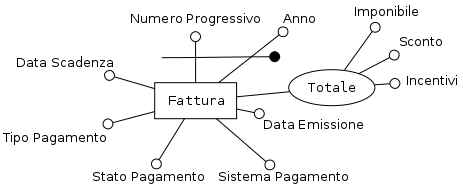
\includegraphics[width=9cm]{images/refactor/fattura.png}
					\centering
					\label{fig:fattura_refactor}
					\caption{Ristrutturazione di \emph{Fattura}}
				\end{figure}

			\paragraph{\emph{Imponibile} in Ordine}
				L'imponibile di un ordine corrisponde al costo delle forniture che lo compongono, su cui vanno calcolate le imposte. La somma di imponibile ed imposte di ordine, indica l'ammontare dell'effettiva transazione monetaria da parte dell'attività al fornitore presso cui è stato effettuato l'ordine.

				Valutiamo la possibilità di aggiungere l'attributo \emph{Imponibile} all'entità \emph{Ordine}.

				\subparagraph{Assenza di Ridondanza}
					Analizziamo il numero di accessi per le operazioni specificate senza introdurre dati ridondanti.

					\vspace{2ex}
					% Nuovo ordine, no ridondanza
					\begin{tabular}{| p{3cm} | p{3cm} | p{3cm} | p{3cm} |}
						\hline
						\multicolumn{4}{|c|}{\textbf{\ref{op:new_ordine}}} \\ \hline
						\textbf{Concetto} & \textbf{Costrutto} & \textbf{Accessi} & \textbf{Tipo} \\ \hline
						Fornitura 	& E & 5 & S \\
						Formazione 	& R & 5 & S \\
						Ordine 		& E & 1 & S \\
						\hline
					\end{tabular}

					% Nuova transazione, no ridondanza
					\begin{tabular}{| p{3cm} | p{3cm} | p{3cm} | p{3cm} |}
						\hline
						\multicolumn{4}{|c|}{\textbf{\ref{op:new_transazione}}} \\ \hline
						\textbf{Concetto} & \textbf{Costrutto} & \textbf{Accessi} & \textbf{Tipo} \\ \hline
						Ordine 		& E & 1 & L \\
						Formazione	& R & 5 & L \\
						Fornitura 	& E & 5 & L \\
						Transazione & E & 1 & S \\
						\hline
					\end{tabular}
					\vspace{2ex}

				\subparagraph{Presenza di Ridondanza}
					Analizziamo ora il numero di accessi introducendo l'attributo \emph{Imponibile} in \emph{Ordine}.

					\vspace{2ex}
					% Nuovo ordine, con ridondanza
					\begin{tabular}{| p{3cm} | p{3cm} | p{3cm} | p{3cm} |}
						\hline
						\multicolumn{4}{|c|}{\textbf{\ref{op:new_ordine}}} \\ \hline
						\textbf{Concetto} & \textbf{Costrutto} & \textbf{Accessi} & \textbf{Tipo} \\ \hline
						Fornitura 	& E & 5 & S \\
						Formazione 	& R & 5 & S \\
						Ordine 		& E & 1 & S \\
						\hline
					\end{tabular}

					% Nuova transazione, con ridondanza
					\begin{tabular}{| p{3cm} | p{3cm} | p{3cm} | p{3cm} |}
						\hline
						\multicolumn{4}{|c|}{\textbf{\ref{op:new_transazione}}} \\ \hline
						\textbf{Concetto} & \textbf{Costrutto} & \textbf{Accessi} & \textbf{Tipo} \\ \hline
						Ordine 		& E & 1 & L \\
						\hline
					\end{tabular}
					\vspace{2ex}

				\subparagraph{Calcolo dei Costi Totali}
					Valutiamo l'introduzione dell'attributo \emph{Imponibile} in \emph{Ordine}.

					\vspace{2ex}
					\begin{tabular}{| p{3cm} | p{3cm} | p{3cm} | p{3cm} |}
						\hline
						\textbf{Operazione} & \textbf{Costo} & \textbf{Frequenza} & \textbf{Totale} \\ \hline
						\ref{op:new_ordine} & 22 & $2 \cdot 4w = 8$ & 176 \\
						\ref{op:new_transazione} & 13 & $2 \cdot 4w = 8$ & 104 \\
						\hline
						\multicolumn{3}{|c|}{\textbf{Costo totale senza ridondanza}} & 280 \\
						\hline
					\end{tabular}

					\begin{tabular}{| p{3cm} | p{3cm} | p{3cm} | p{3cm} |}
						\hline
						\textbf{Operazione} & \textbf{Costo} & \textbf{Frequenza} & \textbf{Totale} \\ \hline
						\ref{op:new_ordine} & 22 & $2 \cdot 4w = 8$ & 176 \\
						\ref{op:new_transazione} & 1 & $2 \cdot 4w = 8$ & 8 \\
						\hline
						\multicolumn{3}{|c|}{\textbf{Costo totale con ridondanza}} & 184 \\
						\hline

					\end{tabular}
					\vspace{2ex}

					Conviene introdurre l'attributo \emph{Imponibile} nell'entità e \emph{Componente}.

					\begin{figure}[H]
						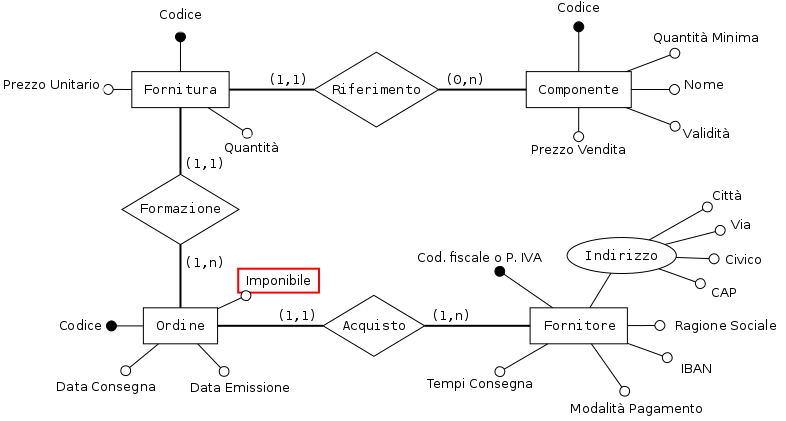
\includegraphics[width=12cm]{images/refactor/fornitore_ordine_fornitura_componente.png}
						\centering
						\label{fig:ordine_refactor}
						\caption{Ristrutturazione di \emph{Ordine}}
					\end{figure}

			\paragraph{\emph{Quantità} in Componente}
				Con \emph{Quantità}, riferito all'entità \emph{Componente}, si intende la quantità degli articoli per uno specifico componente disponibili in magazzino, a prescindere dalla fornitura d'appartenenza.
				Tale definizione fornisce la modalità con cui la quantità presente di un componente può essere calcolata fino a questo momento. Ci occuperemo di stabilire, ora, se possa essere vantaggioso introdurre tale dato derivabile come attributo dell'entità \emph{Componente}.

				\subparagraph{Assenza di Ridondanza}
					Analizziamo gli accessi necessari a svolgere le seguenti operazioni considerando il caso privo di dati ridondanti.

					\vspace{2ex}
					% Consegna ordine, senza ridondanza
					\begin{tabular}{| p{3cm} | p{3cm} | p{3cm} | p{3cm} |}
						\hline
						\multicolumn{4}{|c|}{\textbf{\ref{op:reg_ordine}}} \\ \hline
						\textbf{Concetto} & \textbf{Costrutto} & \textbf{Accessi} & \textbf{Tipo} \\ \hline
						Ordine 		& E & 1 & L \\
						Formazione	& R & 5 & L \\
						Fornitura 	& E & 5 & L \\
						Magazzino  	& E & 5 & S \\
						\hline
					\end{tabular}

					% Controlla componente, no ridondanza
					\begin{tabular}{| p{3cm} | p{3cm} | p{3cm} | p{3cm} |}
						\hline
						\multicolumn{4}{|c|}{\textbf{\ref{op:check_componente}}} \\ \hline
						\textbf{Concetto} & \textbf{Costrutto} & \textbf{Accessi} & \textbf{Tipo} \\ \hline
						Componente 	& E & 1 & L \\
						Magazzino 	& E & 1\footnotemark & L \\
						\hline
					\end{tabular}

					\footnotetext{Valore medio. Per i componenti non presenti in magazzino non ci sarà alcun accesso, per quelli presenti ci saranno tanti accessi quante sono le forniture non ancora esaurite.}

					% Lista componenti presenti, no ridondanza
					\begin{tabular}{| p{3cm} | p{3cm} | p{3cm} | p{3cm} |}
						\hline
						\multicolumn{4}{|c|}{\textbf{\ref{op:list_componenti}}} \\ \hline
						\textbf{Concetto} & \textbf{Costrutto} & \textbf{Accessi} & \textbf{Tipo} \\ \hline
						Magazzino 	& E & $1 \cdot 189=189$ \footnotemark & L \\
						Componente 	& E & $1 \cdot 189=189$ \footnotemark & L \\
						\hline
					\end{tabular}
					\footnotetext{Quantità derivante dalla Tavolta dei Volumi \ref{sec:volume_table}. Sebbene la Tavola dei Volumi sia riferita ad un arco temporale di 3 anni, il volume dell'entità \emph{Magazzino} rimane pressoché costante nel tempo.}
					\footnotetext{Stima massimale. Ad ogni istanza di \emph{Componente} possono corrispondere più istanze di \emph{Magazzino}.}

					% Lista componenti da comprare, no ridondanza
					\begin{tabular}{| p{3cm} | p{3cm} | p{3cm} | p{3cm} |}
						\hline
						\multicolumn{4}{|c|}{\textbf{\ref{op:tobuy_componenti}}} \\ \hline
						\textbf{Concetto} & \textbf{Costrutto} & \textbf{Accessi} & \textbf{Tipo} \\ \hline
						Magazzino 	& E & $1 \cdot 189=189$ & L \\
						Componente 	& E & $1 \cdot 189=189$ & L \\
						\hline
					\end{tabular}
					\vspace{2ex}

				\subparagraph{Presenza di Ridondanza}
					Analizziamo nuovamente il numero di accessi considerando l'attributo ridondante \emph{Quantità}.

					\vspace{2ex}
					% Consegna ordine, con ridondanza
					\begin{tabular}{| p{3cm} | p{3cm} | p{3cm} | p{3cm} |}
						\hline
						\multicolumn{4}{|c|}{\textbf{\ref{op:reg_ordine}}} \\ \hline
						\textbf{Concetto} & \textbf{Costrutto} & \textbf{Accessi} & \textbf{Tipo} \\ \hline
						Ordine 		& E & 1 & L \\
						Formazione	& R & 5 & L \\
						Fornitura 	& E & 5 & L \\
						Magazzino  	& E & 5 & S \\
						Componente 	& E & 1 & L \\
						Componente 	& E & 1 & S \\
						\hline
					\end{tabular}

					% Controlla componente, con ridondanza
					\begin{tabular}{| p{3cm} | p{3cm} | p{3cm} | p{3cm} |}
						\hline
						\multicolumn{4}{|c|}{\textbf{\ref{op:check_componente}}} \\ \hline
						\textbf{Concetto} & \textbf{Costrutto} & \textbf{Accessi} & \textbf{Tipo} \\ \hline
						Componente 	& E & 1 & L \\
						\hline
					\end{tabular}

					% Lista componenti presenti, con ridondanza
					\begin{tabular}{| p{3cm} | p{3cm} | p{3cm} | p{3cm} |}
						\hline
						\multicolumn{4}{|c|}{\textbf{\ref{op:list_componenti}}} \\ \hline
						\textbf{Concetto} & \textbf{Costrutto} & \textbf{Accessi} & \textbf{Tipo} \\ \hline
						Componente 	& E & $1 \cdot 472 = 472$ \footnotemark & L \\
						\hline
					\end{tabular}
					\footnotetext{Dalla Tavola dei Volumi \ref{sec:volume_table}}

					% Lista componenti da comprare, con ridondanza
					\begin{tabular}{| p{3cm} | p{3cm} | p{3cm} | p{3cm} |}
						\hline
						\multicolumn{4}{|c|}{\textbf{\ref{op:tobuy_componenti}}} \\ \hline
						\textbf{Concetto} & \textbf{Costrutto} & \textbf{Accessi} & \textbf{Tipo} \\ \hline
						Componente 	& E & $1 \cdot 472 = 472$ & L \\
						\hline
					\end{tabular}
					\vspace{2ex}

				\subparagraph{Calcolo dei Costi Totali}
					Valutiamo l'introduzione dell'attributo \emph{Quantità} in \emph{Componente}.

					\vspace{2ex}
					\begin{tabular}{| p{3cm} | p{3cm} | p{3cm} | p{3cm} |}
						\hline
						\textbf{Operazione} & \textbf{Costo} & \textbf{Frequenza} & \textbf{Totale} \\ \hline
						\ref{op:reg_ordine}			& 21	& $2 \cdot 4w = 8$		& 168 	\\
						\ref{op:check_componente}	& 2 	& $4 \cdot 24d = 96$	& 192	\\
						\ref{op:list_componenti}	& 378	& $1 \cdot 4w = 4$		& 1512	\\ 
						\ref{op:tobuy_componenti}	& 378	& $1 \cdot 4w = 4$		& 1512	\\
						\hline
						\multicolumn{3}{|c|}{\textbf{Costo totale senza ridondanza}} & 3384 \\
						\hline
					\end{tabular}

					\begin{tabular}{| p{3cm} | p{3cm} | p{3cm} | p{3cm} |}
						\hline
						\textbf{Operazione} & \textbf{Costo} & \textbf{Frequenza} & \textbf{Totale} \\ \hline
						\ref{op:reg_ordine}			& 24	& $2 \cdot 4w = 8$		& 192 	\\
						\ref{op:check_componente}	& 1 	& $4 \cdot 24d = 96$	& 96	\\
						\ref{op:list_componenti}	& 472	& $1 \cdot 4w = 4$		& 1888	\\ 
						\ref{op:tobuy_componenti}	& 472	& $1 \cdot 4w = 4$		& 1888	\\
						\hline
						\multicolumn{3}{|c|}{\textbf{Costo totale con ridondanza}} & 4064 \\
						\hline
					\end{tabular}
					\vspace{2ex}

					L'introduzione dell'attributo \emph{Quantità} in \emph{Componente} aumenterebbe il numero di accessi necessari ad eseguire le operazioni necessarie. Non è necessaria alcuna ristrutturazione.

			\paragraph{\emph{Costo Componenti} in Preventivo}
				L'entità \emph{Componente} è soggetta ad operazioni simili a quelle cui sono soggette le entità \emph{Fattura} ed \emph{Ordine}, quindi è ragionevole valutare l'evenienza di aggiungere il dato derivabile \emph{Costo Componenti}.

				\subparagraph{Assenza di Ridondanza}
					Analizziamo il numero degli accessi necessari per effettuare le operazioni allo stato attuale del modello.

					\vspace{2ex}
					% Nuovo preventivo, no ridondanza
					\begin{tabular}{| p{3cm} | p{3cm} | p{3cm} | p{3cm} |}
						\hline
						\multicolumn{4}{|c|}{\textbf{\ref{op:new_preventivo}}} \\ \hline
						\textbf{Concetto} & \textbf{Costrutto} & \textbf{Accessi} & \textbf{Tipo} \\ \hline
						Preventivo 		& E & 1 & S \\
						Componente 		& E & 6 & L \\
						Previsione		& R & 6 & S \\
						\hline
					\end{tabular}

					% Show preventivo, no ridondanza
					\begin{tabular}{| p{3cm} | p{3cm} | p{3cm} | p{3cm} |}
						\hline
						\multicolumn{4}{|c|}{\textbf{\ref{op:show_preventivi}}} \\ \hline
						\textbf{Concetto} & \textbf{Costrutto} & \textbf{Accessi} & \textbf{Tipo} \\ \hline
						Preventivo 		& E & 1 & L \\
						Previsione		& R & 6 & L \\
						\hline
					\end{tabular}
					\vspace{2ex}

				\subparagraph{Presenza di Ridondanza}
					Vediamo ora il numero di accessi introducendo l'attributo \emph{Costo Componenti} in \emph{Preventivo}.

					\vspace{2ex}
					% Nuovo preventivo, con ridondanza
					\begin{tabular}{| p{3cm} | p{3cm} | p{3cm} | p{3cm} |}
						\hline
						\multicolumn{4}{|c|}{\textbf{\ref{op:new_preventivo}}} \\ \hline
						\textbf{Concetto} & \textbf{Costrutto} & \textbf{Accessi} & \textbf{Tipo} \\ \hline
						Componente 		& E & 6 & L \\
						Preventivo 		& E & 1 & S \\
						Previsione		& R & 6 & S \\
						\hline
					\end{tabular}

					% Show preventivo, con ridondanza
					\begin{tabular}{| p{3cm} | p{3cm} | p{3cm} | p{3cm} |}
						\hline
						\multicolumn{4}{|c|}{\textbf{\ref{op:show_preventivi}}} \\ \hline
						\textbf{Concetto} & \textbf{Costrutto} & \textbf{Accessi} & \textbf{Tipo} \\ \hline
						Preventivo 		& E & 1 & L \\
						\hline
					\end{tabular}
					\vspace{2ex}

				\subparagraph{Calcolo dei Costi Totali}

					Calcoliamo i costi totali nei due casi.

					\vspace{2ex}
					\begin{tabular}{| p{3cm} | p{3cm} | p{3cm} | p{3cm} |}
						\hline
						\textbf{Operazione} & \textbf{Costo} & \textbf{Frequenza} & \textbf{Totale} \\ \hline
						\ref{op:new_preventivo}		& 20 	& $10 \cdot 4w = 40$	& 800	\\
						\ref{op:show_preventivi} 	& 7 	& $2 \cdot 24d = 48$	& 336	\\
						\hline
						\multicolumn{3}{|c|}{\textbf{Costo totale senza ridondanza}} & 1136 \\
						\hline
					\end{tabular}

					\begin{tabular}{| p{3cm} | p{3cm} | p{3cm} | p{3cm} |}
						\hline
						\textbf{Operazione} & \textbf{Costo} & \textbf{Frequenza} & \textbf{Totale} \\ \hline
						\ref{op:new_preventivo}		& 20 	& $10 \cdot 4w = 40$	& 800	\\
						\ref{op:show_preventivi} 	& 1 	& $2 \cdot 24d = 48$	& 48	\\
						\hline
						\multicolumn{3}{|c|}{\textbf{Costo totale con ridondanza}} & 848 \\
						\hline
					\end{tabular}
					\vspace{2ex}

					È conveniente inserire l'attributo ridondante \emph{Costo Componenti} all'entità \emph{Preventivo}, alla luce dei risultati ottenuti.

					\begin{figure}[H]
						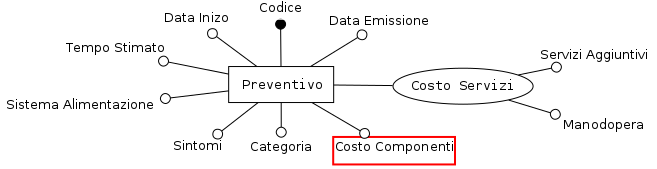
\includegraphics[width=11cm]{images/refactor/preventivo.png}
						\centering
						\label{fig:preventivo_refactor}
						\caption{Ristrutturazione di \emph{Preventivo}}
					\end{figure}

		\subsubsection{Eliminazione delle Generalizzazioni}

			Il modello concettuale, su cui ci stiamo basando in questa fase progettuale, non è ancora adeguato ad essere tradotto in un modello logico. Le generalizzazioni, che con questo passo andremo ad eliminare, sono dei costrutti del modello concettuale che permettono di modellare agevolmente la realtà d'interesse, ma che purtroppo non sono disponibili nel modello relazionale.

			Nel nostro modello concettuale sono presenti due generalizzazioni, quella che coinvolge le entità \emph{Cliente}, \emph{Fornitore} ed \emph{Operatore}, e quella che coinvolge le entità \emph{Privato} ed \emph{Azienda}.

			\begin{description}
				\item [Cliente] 
					Riguardo l'entità \emph{Cliente} abbiamo scelto di accorpare in essa le entità figlie. La motivazione principale sta nel fatto che, effettivamente, le entità figlie non sono direttamente in relazione con nessun'altra parte del modello che fin'ora abbiamo sviluppato.

				\item [Persona]
					Per quanto riguarda le invece le entità figlie di \emph{Persona}, l'accorpamento delle figlie nell'entità padre non è una strada percorribile, sia dal punto di vista tecnico (tale accorpamento genererebbe una tabella troppo corposa, con parecchi valori \emph{NULL}), sia dal punto di vista concettuale (tali entità modellano persone che hanno dei ruoli totalmente diversi tra loro all'interno dell'azienda).

					La scelta che ci sembra più adeguata per questa generalizzazione è quella di accorpare l'entità padre nelle entità figlie, rendendo isolate ed indipendenti tra loro le entità \emph{Cliente}, \emph{Fornitore} e \emph{Operatore}.
			\end{description}

			\begin{figure}[H]
				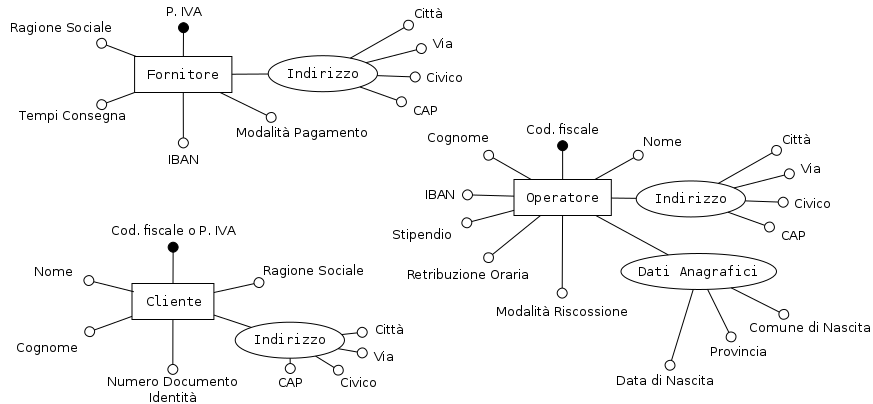
\includegraphics[width=13cm]{images/refactor/persona.png}
				\centering
				\label{fig:preventivo_refactor}
				\caption{Eliminazione delle generalizzazioni}
			\end{figure}
			
		\subsubsection{Partizionamento e Accorpamento di Concetti}

			\paragraph{Partizionamento di Concetti}
				L'eliminazione dell'entità padre \emph{Persona} induce un partizionamento della relationship \emph{Rubrica} con la quale veniva associata all'entità \emph{Recapito}.

				Il partizionamento più naturale per tale relationship ricalca il concetto della separazione delle entità \emph{Cliente}, \emph{Fornitore} e \emph{Operatore} effettuata nel precedente passo.

				Tale relationship sarà sostituita da tre relationship distinte (figura \ref{fig:rubrica_refactor}): \emph{Rubrica Cliente}, \emph{Rubrica Fornitore} e \emph{Rubrica Operatore}.

				\begin{sidewaysfigure}
					\centering
					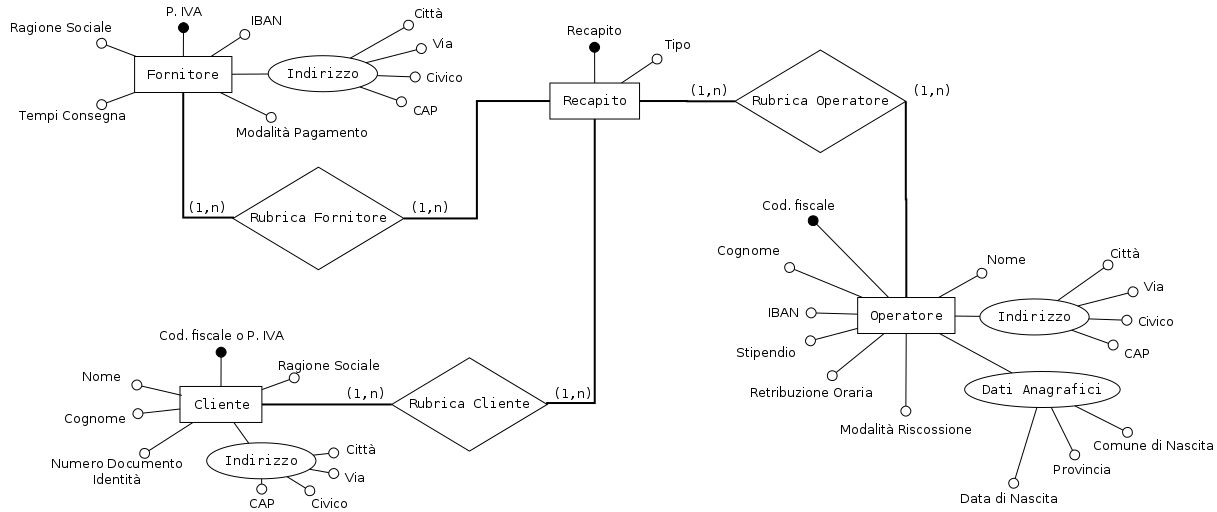
\includegraphics[width=22cm]{images/refactor/persona-recapito.png}
					\caption{Partizionamento di Rubrica}
					\label{fig:rubrica_refactor}
				\end{sidewaysfigure}

	\subsection{Scelta degli Identificatori Principali}

		Per quanto possibile, abbiamo scelto degli identificatori primari che fossero il più possibile significativi per ognuna delle entità. Purtroppo non abbiamo trovato degli identificativi, per così dire, \emph{naturali} tra gli attributi delle entità quali \emph{Componente}, \emph{Preventivo}, \emph{Fornitura} ed \emph{Ordine}, dovendo introdurre dei codici identificativi interni.

		Per alcune entità, come \emph{Fattura} e \emph{Magazzino}, mantenuto le superchiavi evitando di aggiungere altri attributi \emph{Codice}, con il fine di mantenere le rappresentazioni dei concetti che modellano, fedeli alla realtà.

		Per quanto riguarda invece l'entità \emph{Turno}, sembrava effettivamente superfluo e poco intuitivo insierire un attributo che fungesse da identificatore primario.

		In figura \ref{fig:schema_refactor} troviamo l'intero modello ER alla fine della sua ristrutturazione.
		
		\vspace{2ex}
		\begin{longtable}{| p{6.2cm} | p{6.2cm} |}
			\hline
			\textbf{Nome Entità} & \textbf{Identificatore} \\
			\hline
			\endfirsthead

			\hline
			\textbf{Nome Entità} & \textbf{Identificatore} \\
			\hline
			\endhead

			Cliente 		& Codice Fiscale o P.IVA 	\\ \hline
			Fornitore 		& Partita IVA 				\\ \hline
			Operatore 		& Codice Fiscale 			\\ \hline
			Autovettura  	& Targa						\\ \hline
			Preventivo 		& Codice					\\ \hline
			Componente 		& Codice					\\ \hline
			Fornitura 		& Codice					\\ \hline
			Ordine 			& Codice					\\ \hline
			Magazzino  		& Codice Componente, Codice (di \emph{Fornitura}			\\ \hline
			Prestazione 	& Codice (di \emph{Preventivo})								\\ \hline
			Turno			& Ora Inizio, Data, Codice Fiscale (di \emph{Operatore})	\\ \hline
			Transazione 	& Codice					\\ \hline
			Fattura         & Numero Progressivo, Anno 	\\ \hline
			Recapito 		& Recapito 					\\ \hline

			\hline			
		\end{longtable}
		\vspace{2ex}

		\begin{sidewaysfigure}
			\centering
			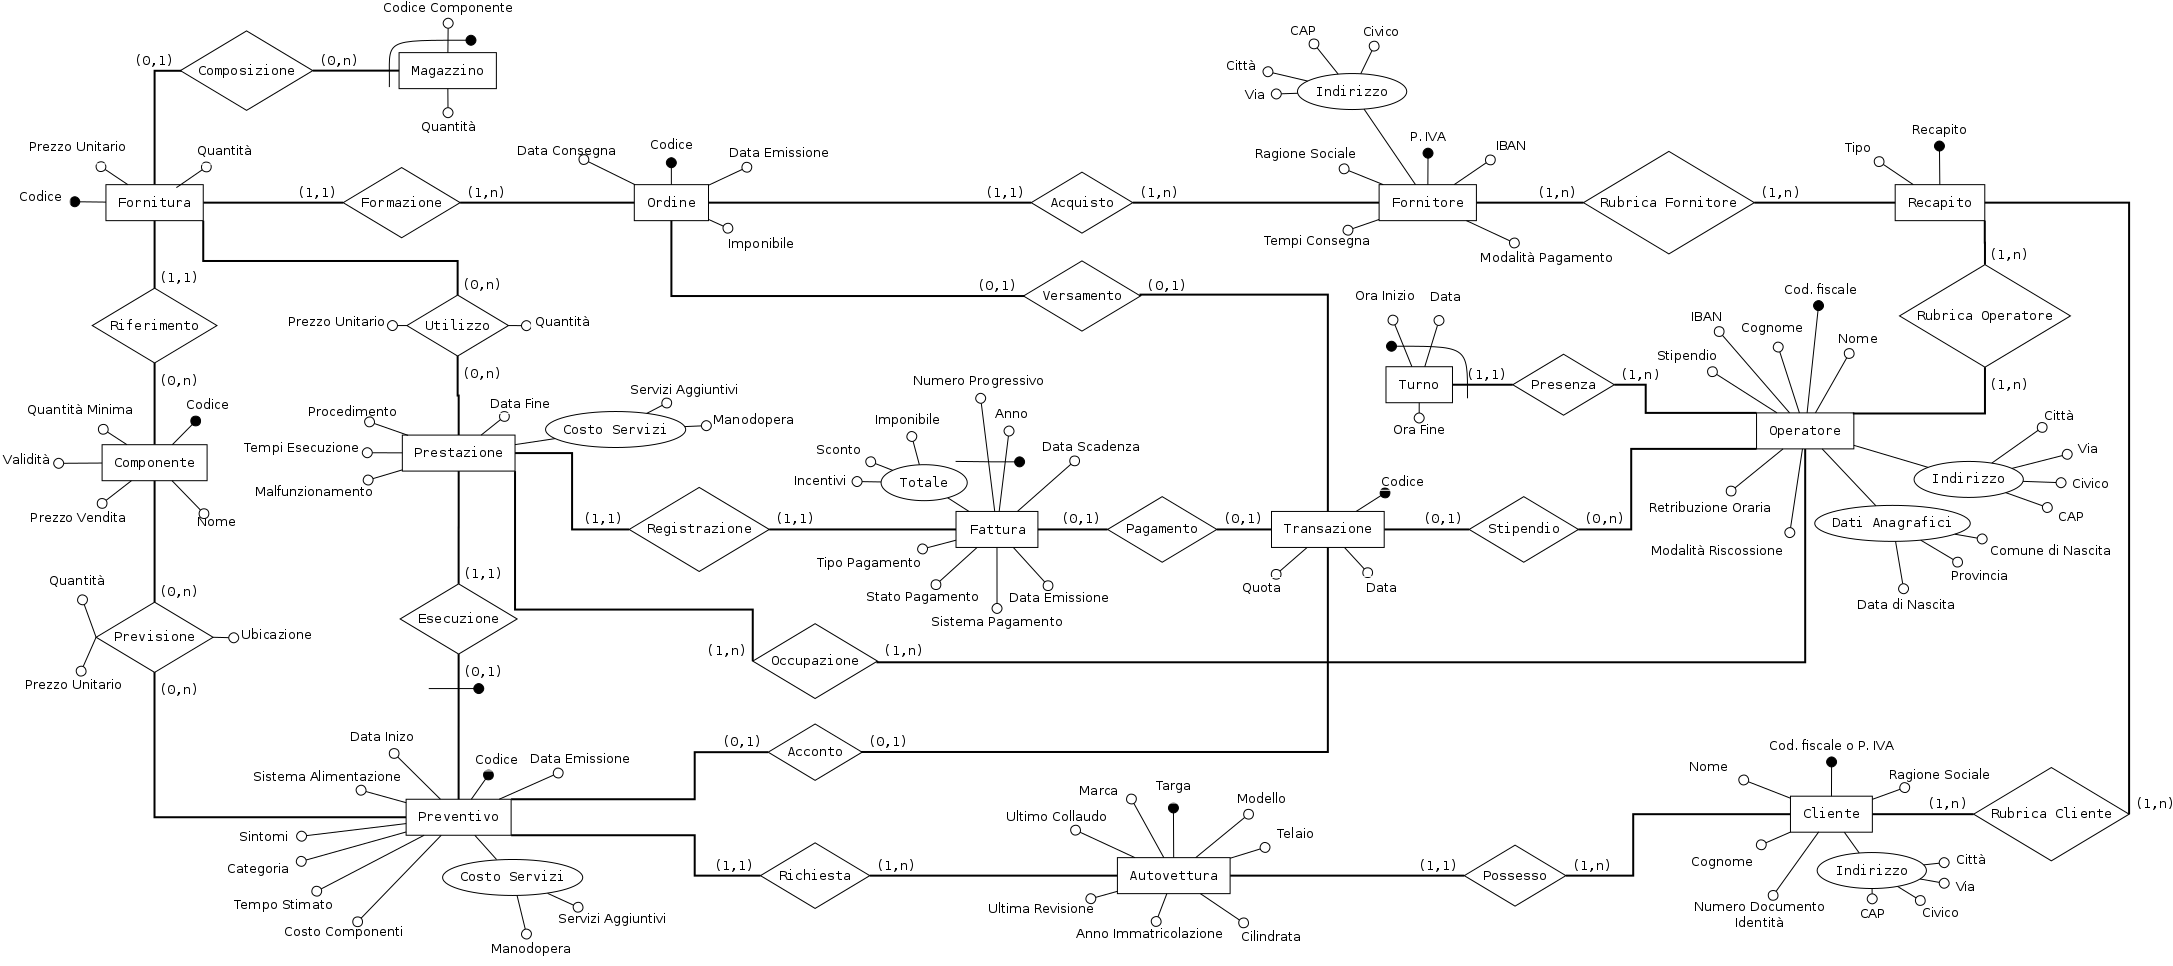
\includegraphics[width=22cm]{images/refactor/schema.png}
			\caption{Diagramma Entity-Relationship Ristrutturato}
			\label{fig:schema_refactor}
		\end{sidewaysfigure}

	\subsection{Normalizzazione}
		Da mettere prima o dopo la traduzione verso il modello relazionale
	\subsection{Traduzione verso il Modello Relazionale}

\newpage

% Sezione con gli screenshot delle chiamate alla base di dati
%!TEX root = Progetto.tex
\section{Codifica Sql e Testing} % (fold)
\label{sec:codifica_sql_e_testing}

Di seguito è riportata la definizione dello schema in linguaggio sql così come è implementato nel dump. Si allegano, per ogni tabella, degli screenshot dal terminale.

Il DBMS utilizzato (MySQL 5) nativamente non supporta la definizione di vincoli d'integrità personalizzabili. Per ovviare a questa limitazione, nell'implementazione completa dello schema (riportata nel dump) si è fatto un larghissimo uso di trigger che implementano la logica dei vincoli.

	\subsection{Definizione dello schema e screenshot successivi all'inserimento di dati}
		% Cliente

		\pagebreak
	\subsection{Codifica delle operazioni}
		Di seguito vengono riportate le implementazioni delle operazioni effettuabili sulla base di dati. La loro organizzazione non è lineare come l'elenco presentato in fase progettuale, ma rispecchia quelli che sono i reali casi d'uso.

		\begin{enumerate}

			\item Inserimento di un nuovo cliente. A tale inserimento corrisponde sempre l'inserimento e l'associazione di una nuova autovettura e di almeno un recapito.
			\begin{lstlisting}
/** Cliente non dotato di partita iva */
INSERT INTO Cliente (CF_PIVA, Nome, Cognome, Citta, 
	Via, Civico, CAP, NDocId) 
VALUES (...);

/** Cliente dotato di partita iva */
INSERT INTO Cliente (CF_PIVA, RagioneSociale, Citta, 
	Via, Civico, CAP) 
VALUES (...);

/** Inserimento dell'autovettura */
INSERT INTO Autovettura (Targa, Telaio, Marca, Modello, 
	Cilindrata, AnnoImmatricolazione, UltimoCollaudo, 
	UltimaRevisione, Cliente) 
VALUES (..., <CF_PIVA del cliente appena inserito>);

/** Inserimento di un recapito */
INSERT INTO Recapito (Recapito, Tipo)
VALUES (...);

/** Associazione di un recapito inserito al cliente */
INSERT INTO RubricaCliente (Recapito, Cliente)
VALUES (<Codice del recapito>, <CF_PIVA del cliente>);
				\end{lstlisting}

			L'aggiunta di un recapito ad un cliente è un'operazione molto frequente. Per questo è stata creata una procedura che si occupa dell'inserimento e dell'associazione dello stesso:
				\begin{lstlisting}
CREATE PROCEDURE add_recapito_cliente(
  IN cf_piva  VARCHAR(16),
     recapito VARCHAR(200),
     tipo     ENUM('telefono',
                   'fax',
                   'tel_fax',
                   'sito_web',
                   'email')
)
  BEGIN
    DECLARE EXIT HANDLER FOR SQLEXCEPTION
    BEGIN
      ROLLBACK;
      /* La procedura throw_error si occupa di lanciare 
       * un segnale d'errore con codice 45000
       * e con il messaggio specificato come argomento
       */
      CALL throw_error('Recapito già registrato');
    END;
    START TRANSACTION;
    INSERT INTO Recapito (Recapito, Tipo) VALUES (recapito, tipo);
    SELECT LAST_INSERT_ID()
    INTO @last_id;
    INSERT INTO RubricaCliente (Recapito, Cliente) VALUES (@last_id, cf_piva);
    COMMIT;
  END;;
				\end{lstlisting}

			\item Inserimento di un nuovo fornitore. All'inserimento di un nuovo fornitore corrisponde l'inserimento dei relativi recapiti.
			\begin{lstlisting}
/** Inserimento del fornitore */
INSERT INTO Fornitore (PIVA, RagioneSociale, TempiConsegna,
	ModPagamento, IBAN, Citta, Via, Civico, CAP) 
VALUES (...);

/** Associazione di un recapito inserito al fornitore
	(L'operazione di inserimento di un nuovo recapito
	è identica a quella presentata nel caso d'uso 
	precedente) */
INSERT INTO RubricaFornitore (Recapito, Fornitore)
VALUES (<Codice del recapito>, <PIVA del fornitore>);
			\end{lstlisting}

			Come nel caso precedente, anche per il fornitore esiste una procedura per l'aggiunta e l'associazione di un recapito.
			Gli inserimenti diventano molto più compatti:
			\begin{lstlisting}
CALL add_recapito_fornitor(<PIV del fornitore>,
	<recapito>, <tipo del recapito>);
			\end{lstlisting}

			\item Inserimento di un nuovo operatore. Anche in questo caso bisognerà aggiungere uno o più recapiti a quest'ultimo. Presentiamo inoltre anche l'istruzione per inserire un nuovo turno di lavoro.
			\begin{lstlisting}
/** Inserimento di un operatore con stipendio fisso */
INSERT INTO Operatore (CF, Nome, Cognome, Citta, Via, 
	Civico, CAP, DataNasc, ComuneNasc, ProvinciaNasc, 
	Stipendio, ModRiscossione, IBAN)
VALUES (...);

/** Inserimento di un operatore con retribuzione
	oraria */
INSERT INTO Operatore (CF, Nome, Cognome, Citta, Via,
	Civico, CAP, DataNasc, ComuneNasc, ProvinciaNasc, 
	RetribuzioneH, ModRiscossione, IBAN)
VALUES (...);

/** Inserimento di un nuovo turno di lavoro */
INSERT INTO Turno (Operatore, Data, OraInizio, OraFine)
VALUES (<CF dell'operatore>, ...);
			\end{lstlisting}

			\item Registrazione di un nuovo componente.
			\begin{lstlisting}
INSERT INTO Componente (Nome, QuantitaMin, Validita, 
	PrezzoVendita) 
VALUES (...);
			\end{lstlisting}

			\item Inserimento di un nuovo ordine. Questa operazione si articola in più parti: innanzi tutto bisogna creare una nuova istanza nella relazione \emph{Ordine}, quindi creare le istanze relative alle forniture dell'ordeine, aggiornare il magazzino ed inserire una nuova transazione a pagamento avvenuto dell'ordine.

			\begin{lstlisting}

			\end{lstlisting}

		\end{enumerate}

\end{document}
